
\subsubsection{Análisis para $R_{comp}$ en modo tensión, $V_{out} = 10 \si[per-mode=symbol]{\volt}$, $R_{L} = 10 \si[per-mode=symbol]{\ohm}$}

Se puede ver en la figura~\figref{fig:fig_power_supply_RCOMP_LOOP_Modo1} como ya con el valor de $R_{comp} = 10 \si[per-mode=symbol]{\ohm}$ se logra unos margen de fase y ganancia muy buenos, valores de $R_{comp}$ por debajo o por arriba o empeoran los márgenes o presentan picos de resonancia en la respuesta en frecuencia, además que un valor mayor disminuye el ancho de banda, como se puede ver en la figura~\figref{fig:fig_power_supply_RCOMP_RF_Modo1}. A nivel de respuesta dinámica, se ve que un valor mayor genera un mayor sobre-pico, asociado al pico observado en la ganancia de lazo, ver figura~\figref{fig:fig_power_supply_RCOMP_STEP_0_Modo1}, figura~\figref{fig:fig_power_supply_RCOMP_STEP_10_Modo1} y figura~\figref{fig:fig_power_supply_RCOMP_STEP_100_Modo1}.

\vfill


% RCOMP MODO 1.

\clearpage

\begin{figure}[H] %htb
\begin{center}
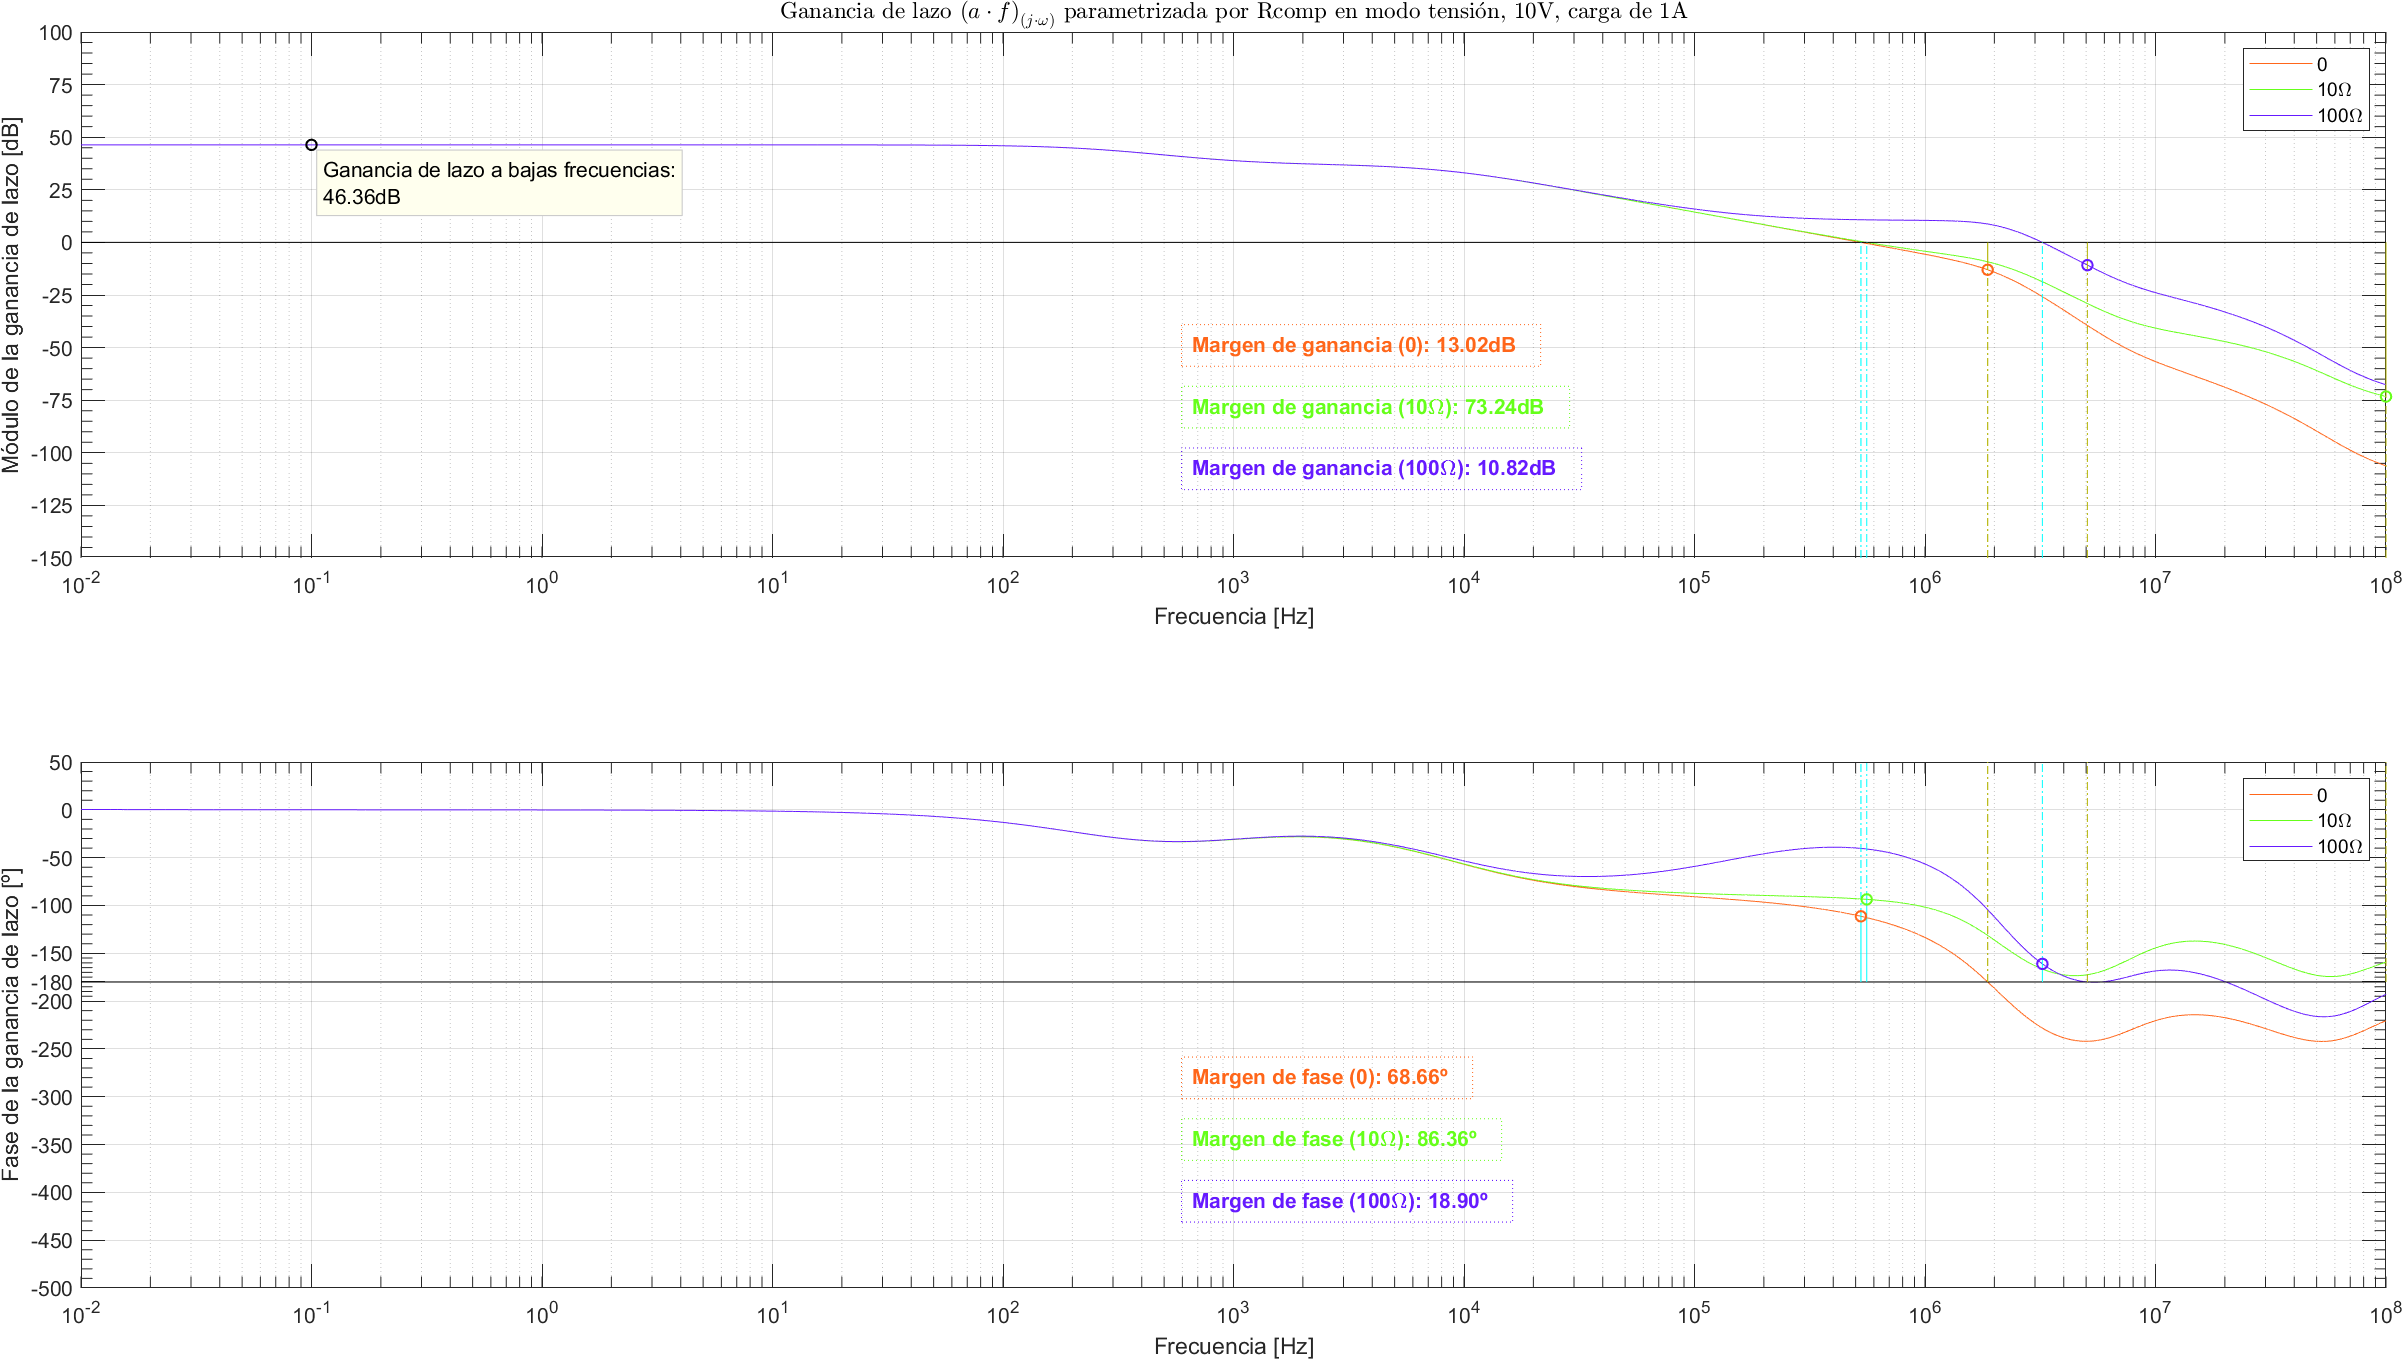
\includegraphics[width=1.1 \textwidth, angle=90]{./img/plots/loop/power_supply_RCOMP_LOOP_Modo1.png}
\caption{\label{fig:fig_power_supply_RCOMP_LOOP_Modo1}\footnotesize{Ganancia de lazo en modo tensión, $V_{out} = 10 \si[per-mode=symbol]{\volt}$, en función de la frecuencia parametrizada por $R_{comp}$.}}
\end{center}
\end{figure}


\clearpage

\begin{figure}[H] %htb
\begin{center}
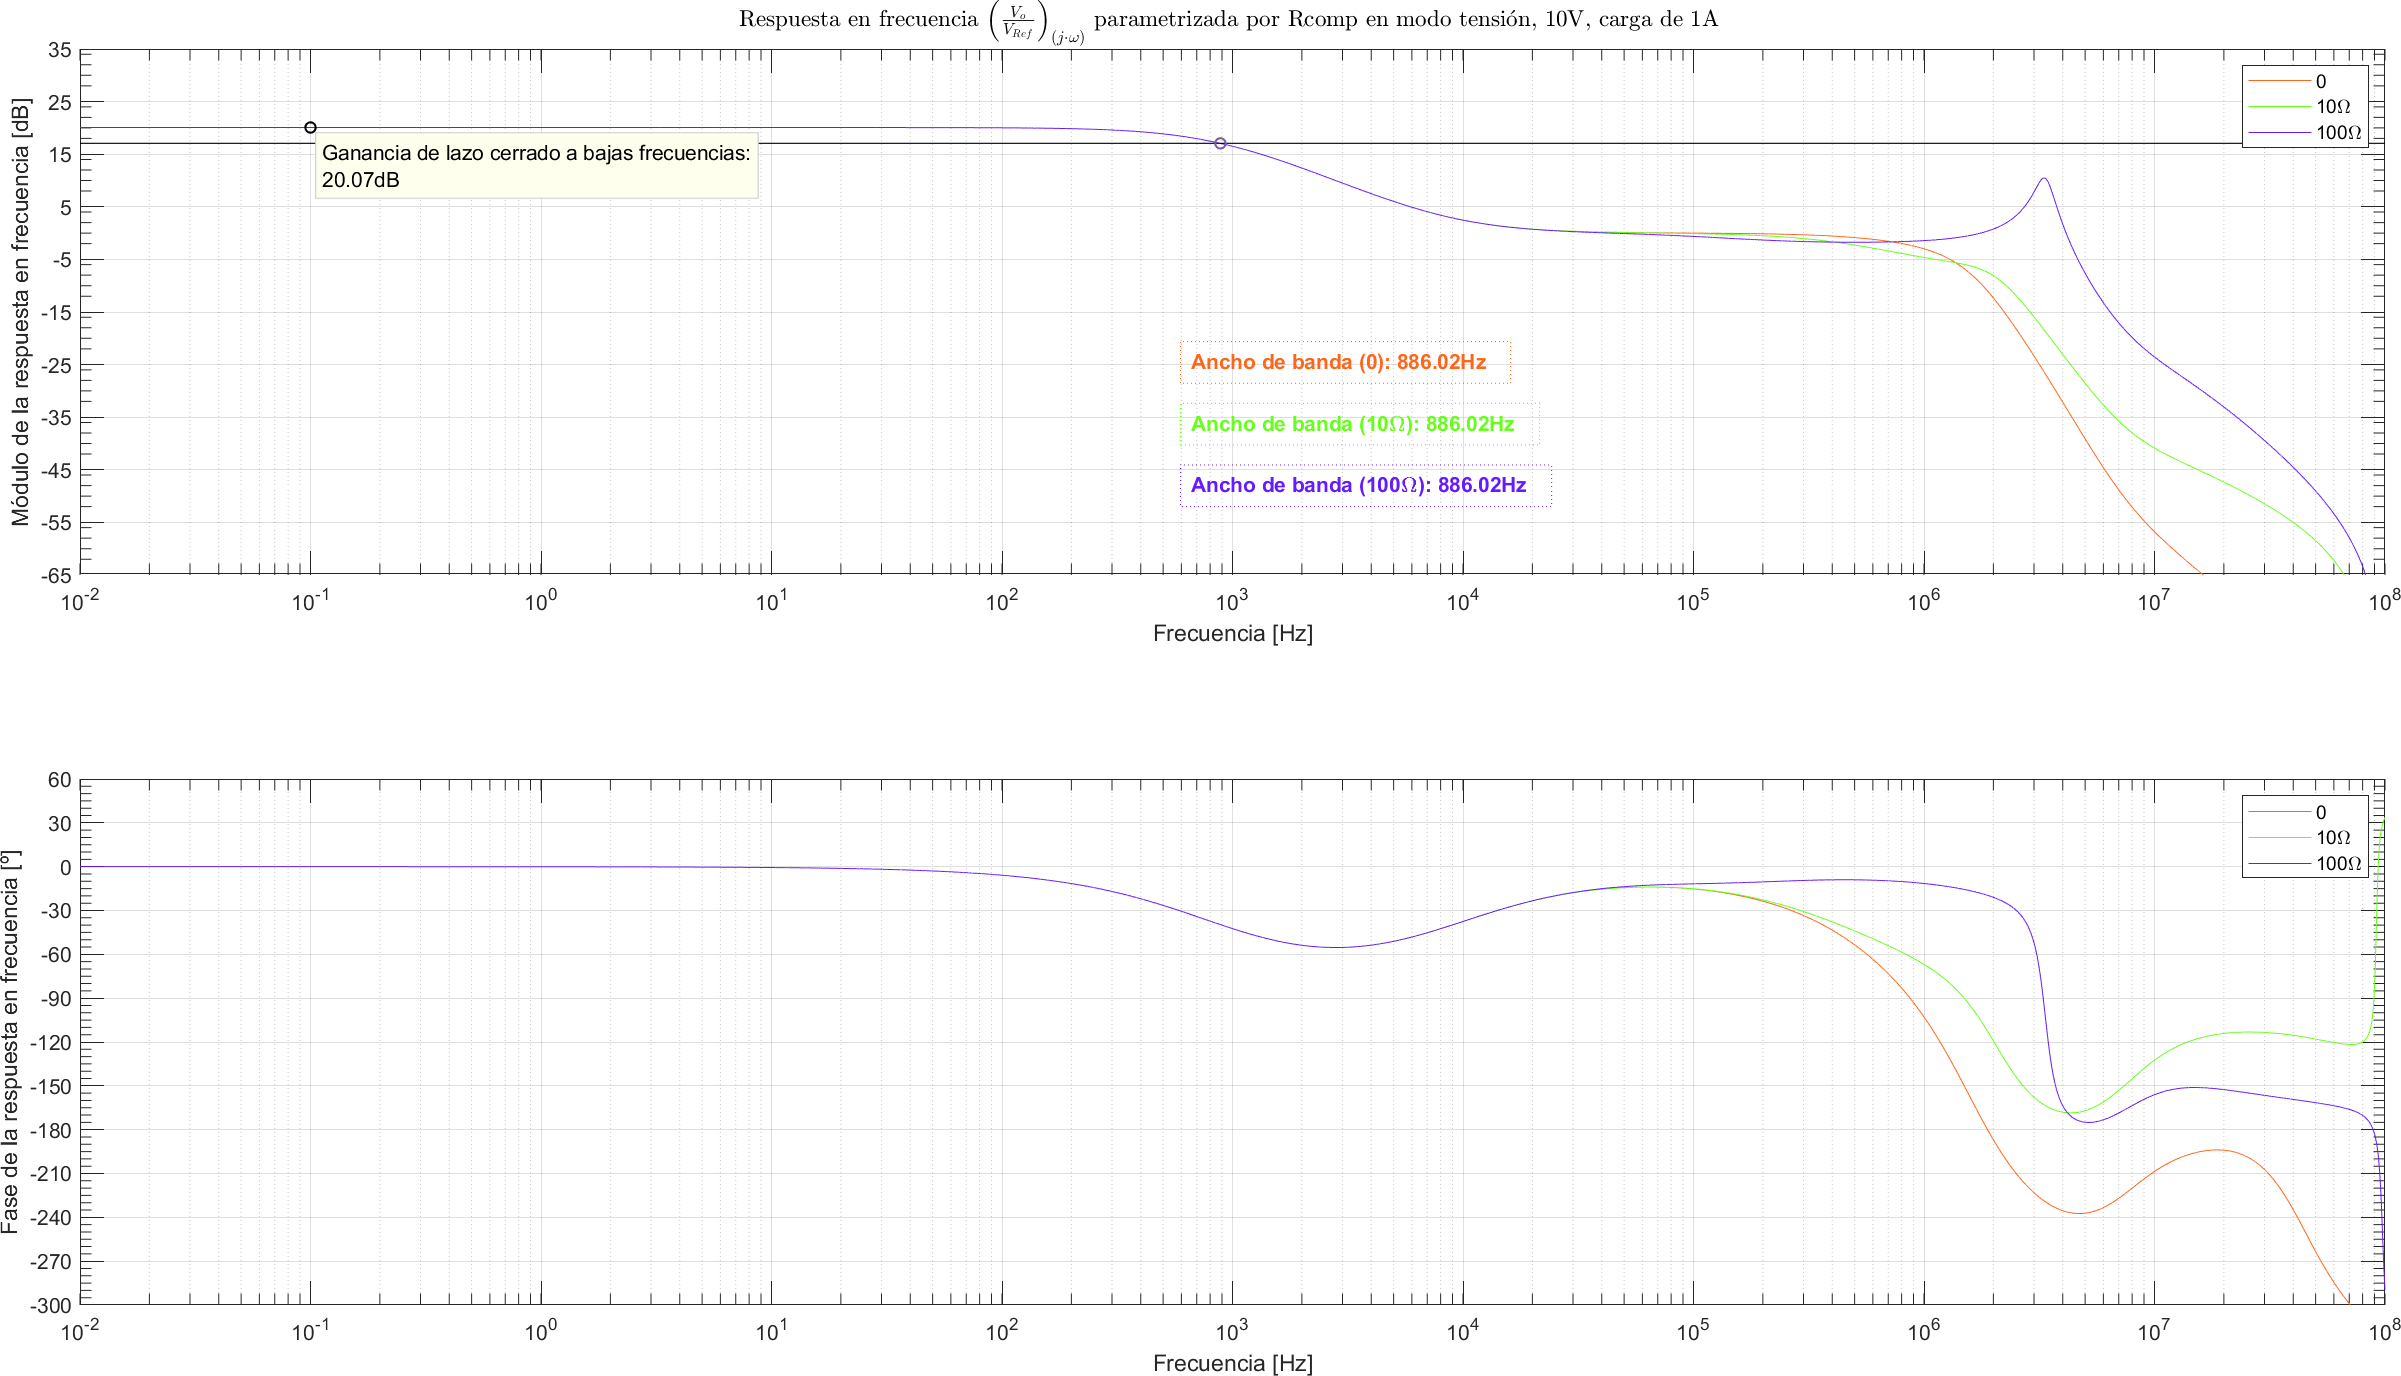
\includegraphics[width=1.1 \textwidth, angle=90]{./img/plots/rf/power_supply_RCOMP_RF_Modo1.png}
\caption{\label{fig:fig_power_supply_RCOMP_RF_Modo1}\footnotesize{Respuesta en frecuencia en modo tensión, $V_{out} = 10 \si[per-mode=symbol]{\volt}$, en función de la frecuencia parametrizada por $R_{comp}$.}}
\end{center}
\end{figure}

\clearpage

\begin{figure}[H] %htb
\begin{center}
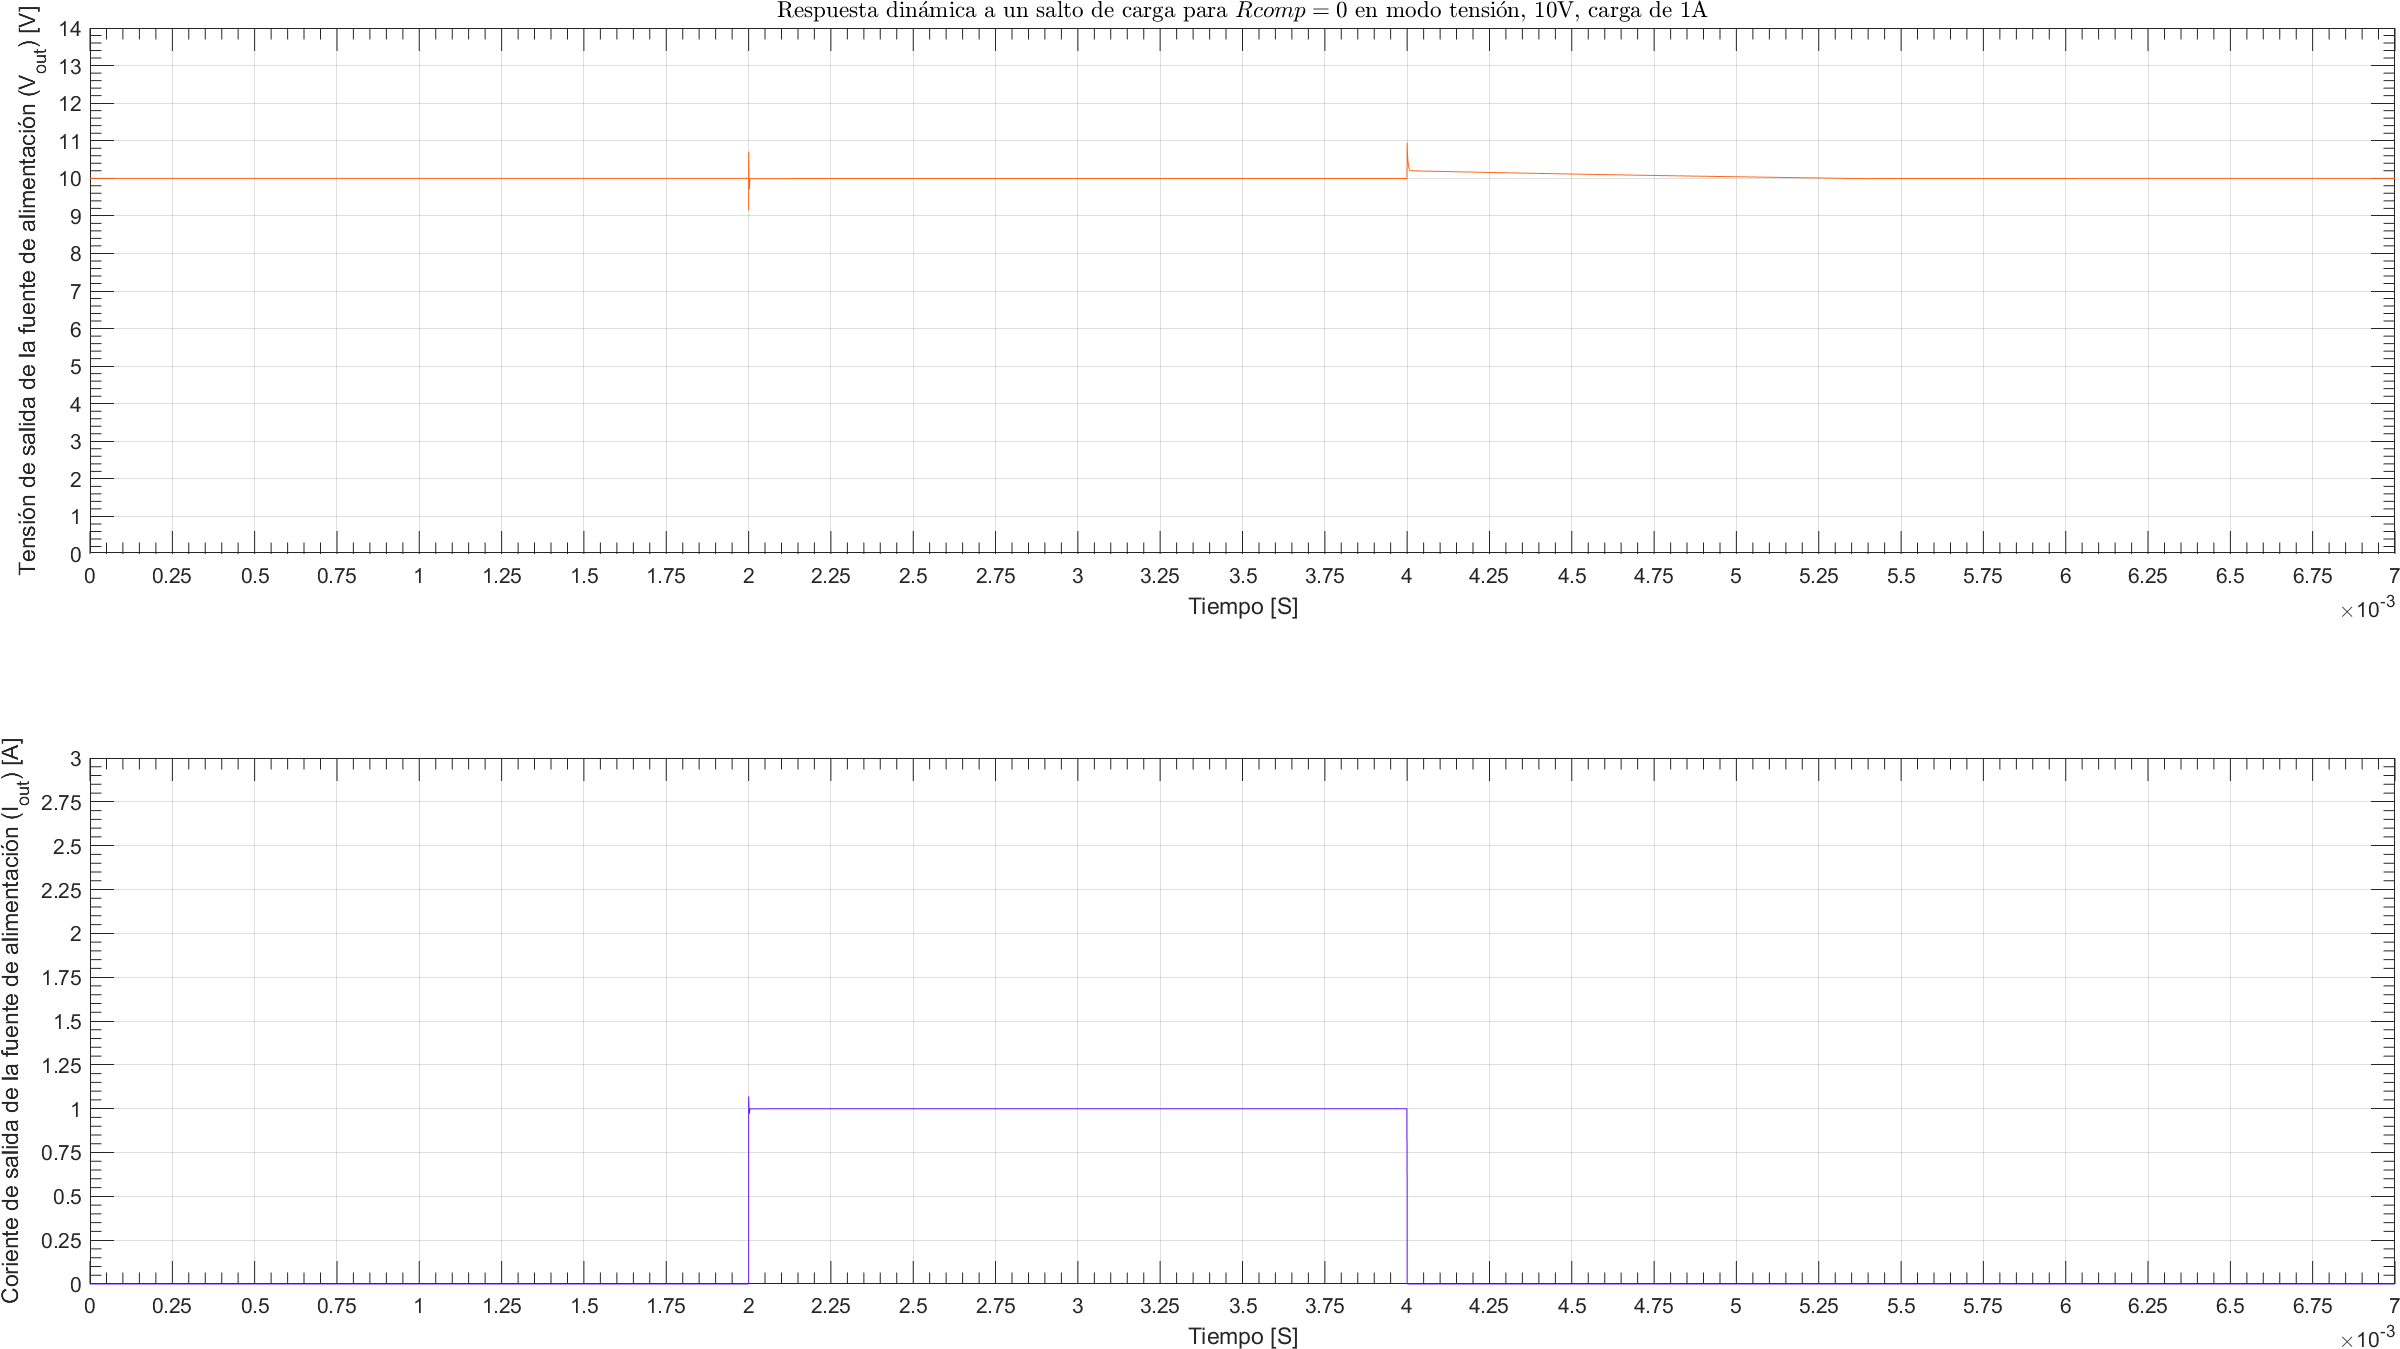
\includegraphics[width=1.1 \textwidth, angle=90]{./img/plots/dynamic/power_supply_RCOMP_0_STEP_Modo1.png}
\caption{\label{fig:fig_power_supply_RCOMP_STEP_0_Modo1}\footnotesize{Respuesta dinámica en modo tensión, $V_{out} = 10 \si[per-mode=symbol]{\volt}$, para $R_{comp} = 0 \si[per-mode=symbol]{\ohm} $.}}
\end{center}
\end{figure}

\clearpage

\begin{figure}[H] %htb
\begin{center}
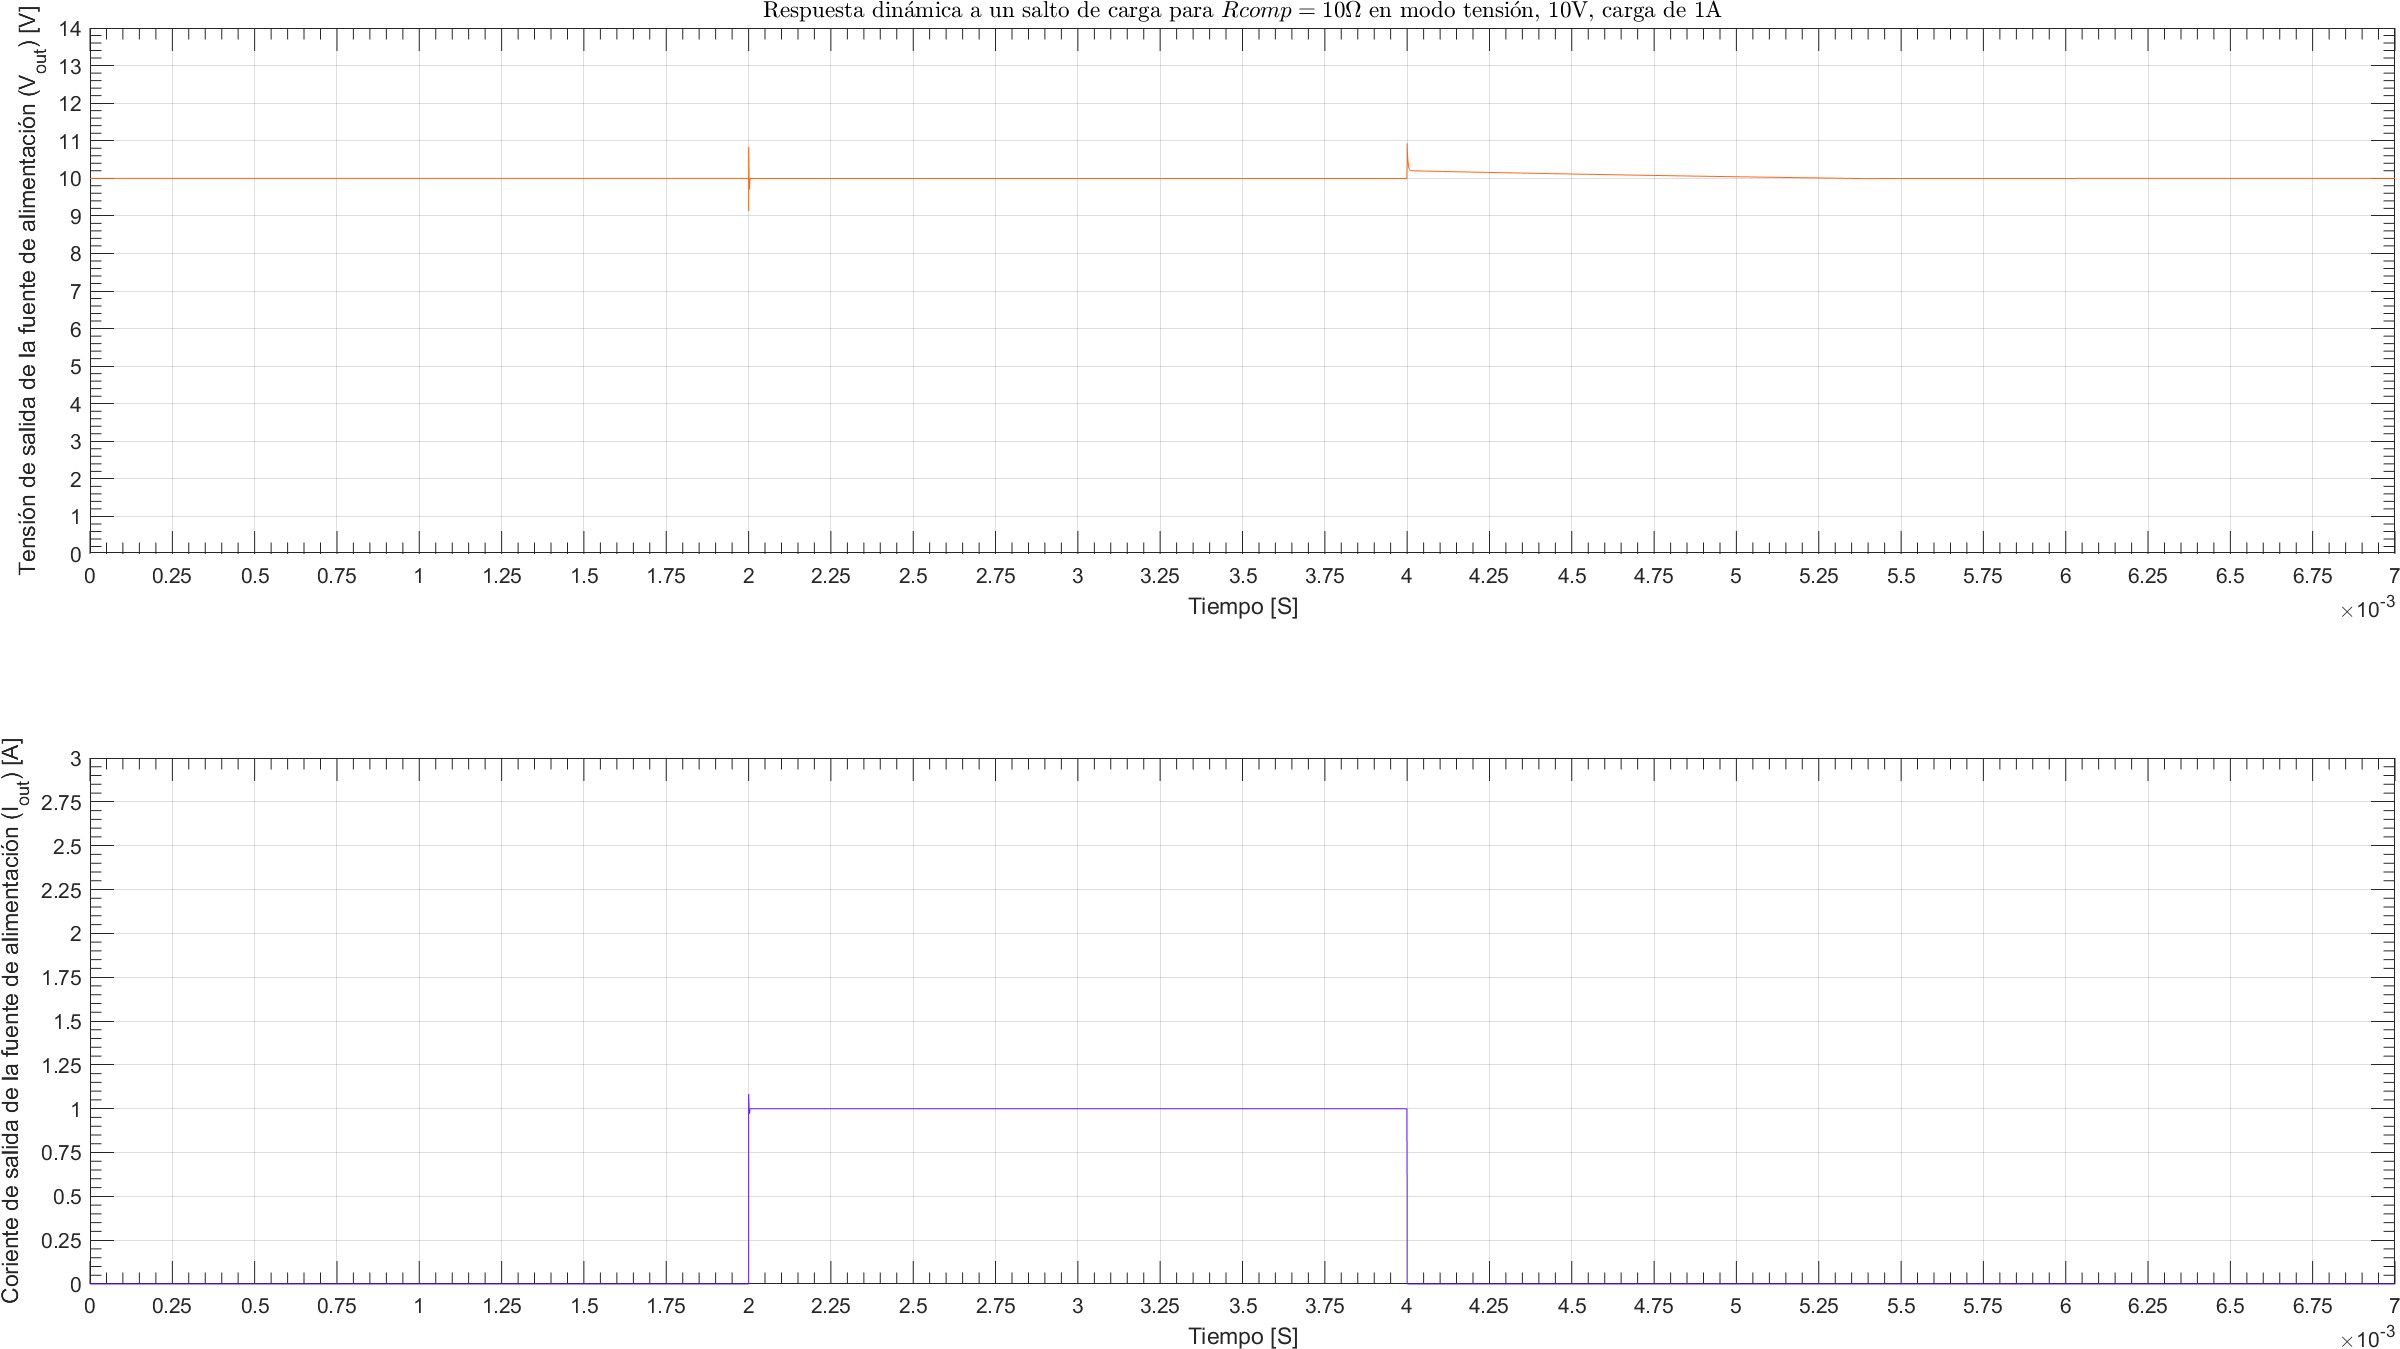
\includegraphics[width=1.1 \textwidth, angle=90]{./img/plots/dynamic/power_supply_RCOMP_10_STEP_Modo1.png}
\caption{\label{fig:fig_power_supply_RCOMP_STEP_10_Modo1}\footnotesize{Respuesta dinámica en modo tensión, $V_{out} = 10 \si[per-mode=symbol]{\volt}$, para $R_{comp} = 10 \si[per-mode=symbol]{\ohm} $.}}
\end{center}
\end{figure}

\clearpage

\begin{figure}[H] %htb
\begin{center}
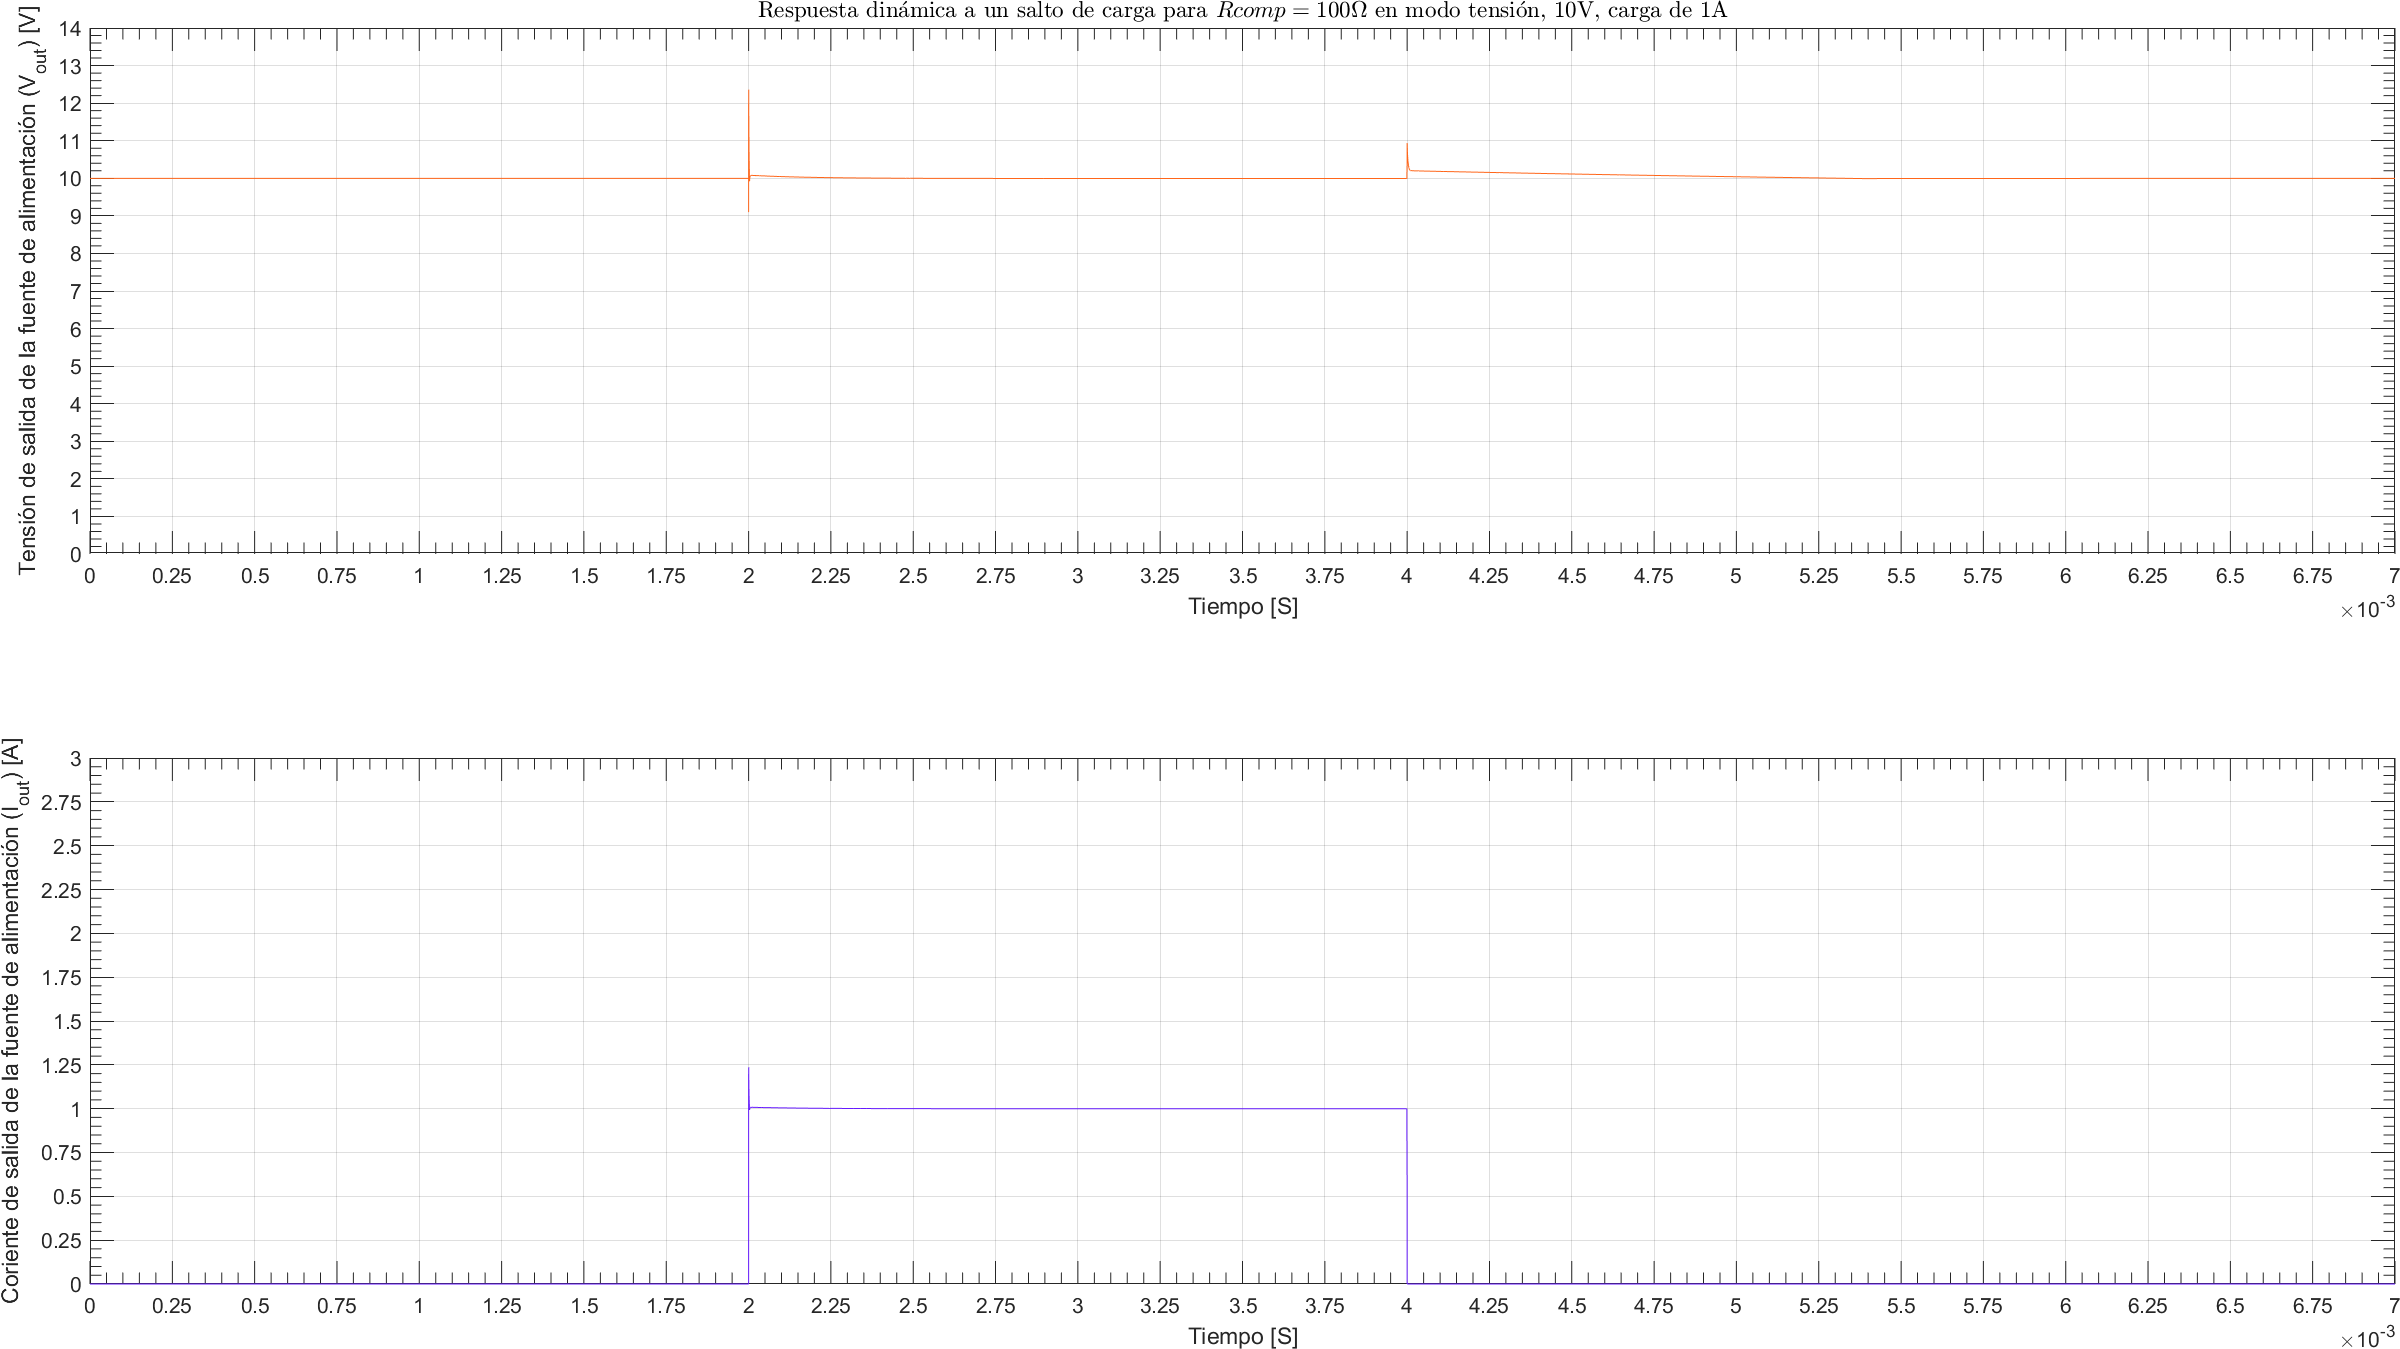
\includegraphics[width=1.1 \textwidth, angle=90]{./img/plots/dynamic/power_supply_RCOMP_100_STEP_Modo1.png}
\caption{\label{fig:fig_power_supply_RCOMP_STEP_100_Modo1}\footnotesize{Respuesta dinámica en modo tensión, $V_{out} = 10 \si[per-mode=symbol]{\volt}$, para $R_{comp} = 100 \si[per-mode=symbol]{\ohm} $.}}
\end{center}
\end{figure}

\clearpage


\subsubsection{Análisis para $R_{comp}$ en modo tensión, $V_{out} = 1 \si[per-mode=symbol]{\volt}$, $R_{L} = 1 \si[per-mode=symbol]{\ohm}$}

Se puede ver en la figura~\figref{fig:fig_power_supply_RCOMP_LOOP_Modo2} como ya con el valor de $R_{comp} = 10 \si[per-mode=symbol]{\ohm}$ se logra unos margen de fase y ganancia muy buenos, valores de $R_{comp}$ por debajo o por arriba o empeoran los márgenes o presentan picos de resonancia en la respuesta en frecuencia, además que un valor mayor disminuye el ancho de banda, como se puede ver en la figura~\figref{fig:fig_power_supply_RCOMP_RF_Modo2}. A nivel de respuesta dinámica, se ve que un valor mayor genera un mayor sobre-pico, asociado al pico observado en la ganancia de lazo, ver figura~\figref{fig:fig_power_supply_RCOMP_STEP_0_Modo2}, figura~\figref{fig:fig_power_supply_RCOMP_STEP_10_Modo2} y figura~\figref{fig:fig_power_supply_RCOMP_STEP_100_Modo2}.

\vfill


% RCOMP MODO 2.

\clearpage

\begin{figure}[H] %htb
\begin{center}
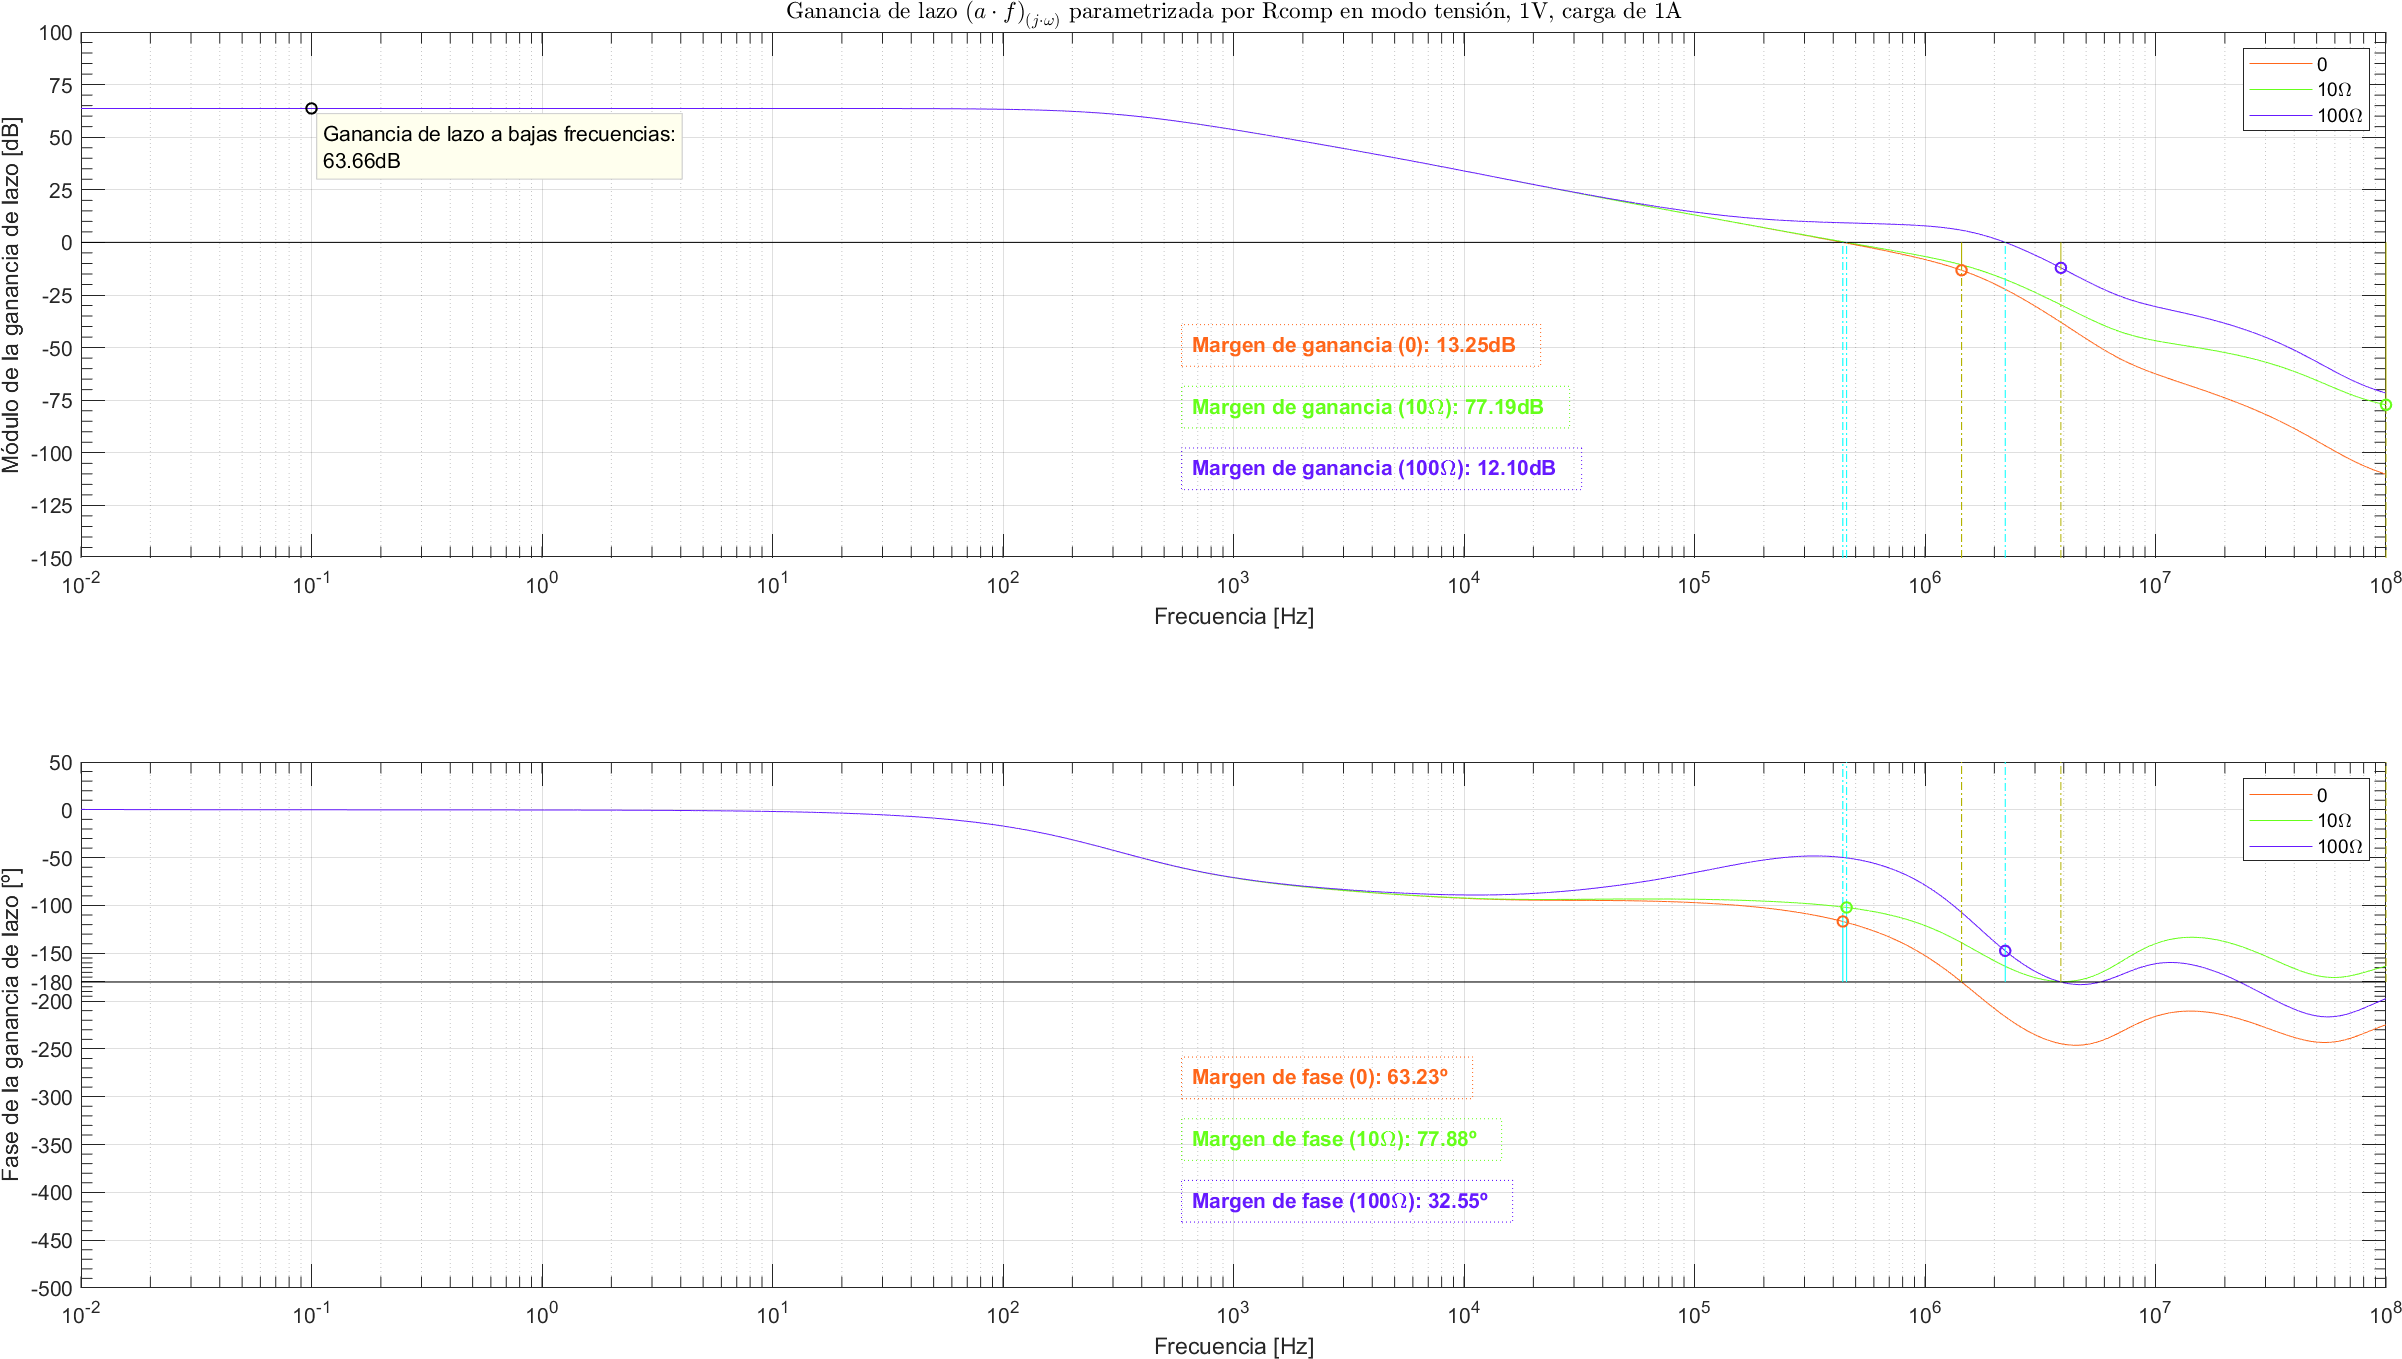
\includegraphics[width=1.1 \textwidth, angle=90]{./img/plots/loop/power_supply_RCOMP_LOOP_Modo2.png}
\caption{\label{fig:fig_power_supply_RCOMP_LOOP_Modo2}\footnotesize{Ganancia de lazo en modo tensión, $V_{out} = 1 \si[per-mode=symbol]{\volt}$, en función de la frecuencia parametrizada por $R_{comp}$.}}
\end{center}
\end{figure}


\clearpage

\begin{figure}[H] %htb
\begin{center}
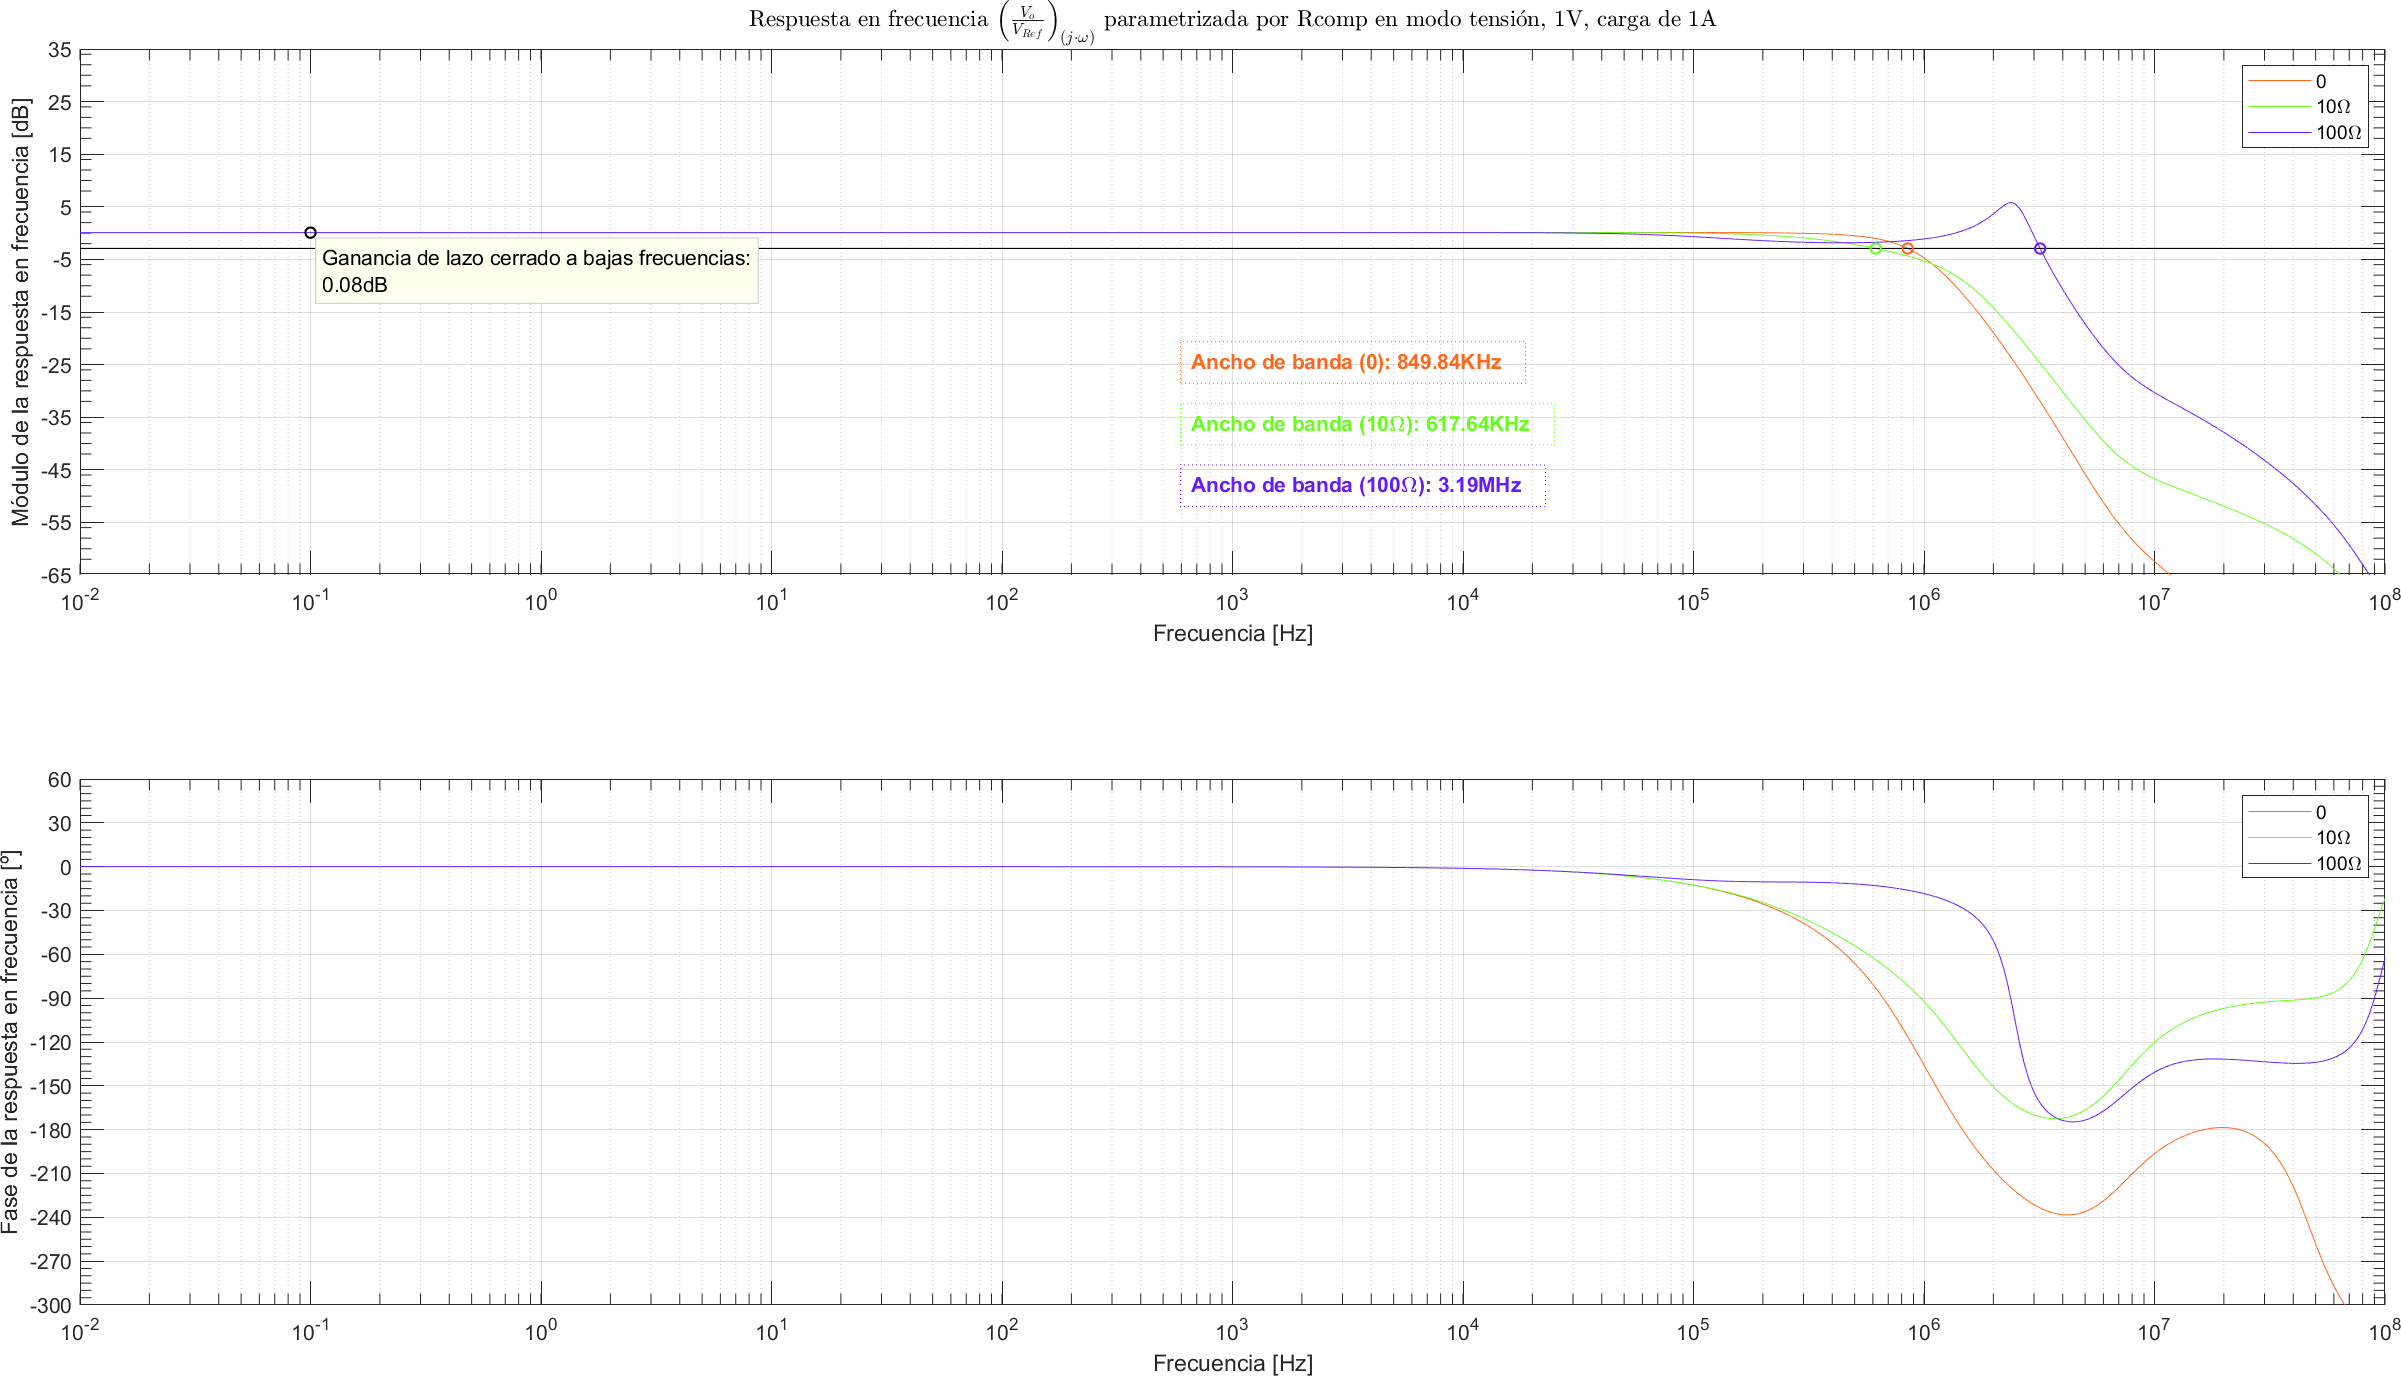
\includegraphics[width=1.1 \textwidth, angle=90]{./img/plots/rf/power_supply_RCOMP_RF_Modo2.png}
\caption{\label{fig:fig_power_supply_RCOMP_RF_Modo2}\footnotesize{Respuesta en frecuencia en modo tensión, $V_{out} = 1 \si[per-mode=symbol]{\volt}$, en función de la frecuencia parametrizada por $R_{comp}$.}}
\end{center}
\end{figure}

\clearpage

\begin{figure}[H] %htb
\begin{center}
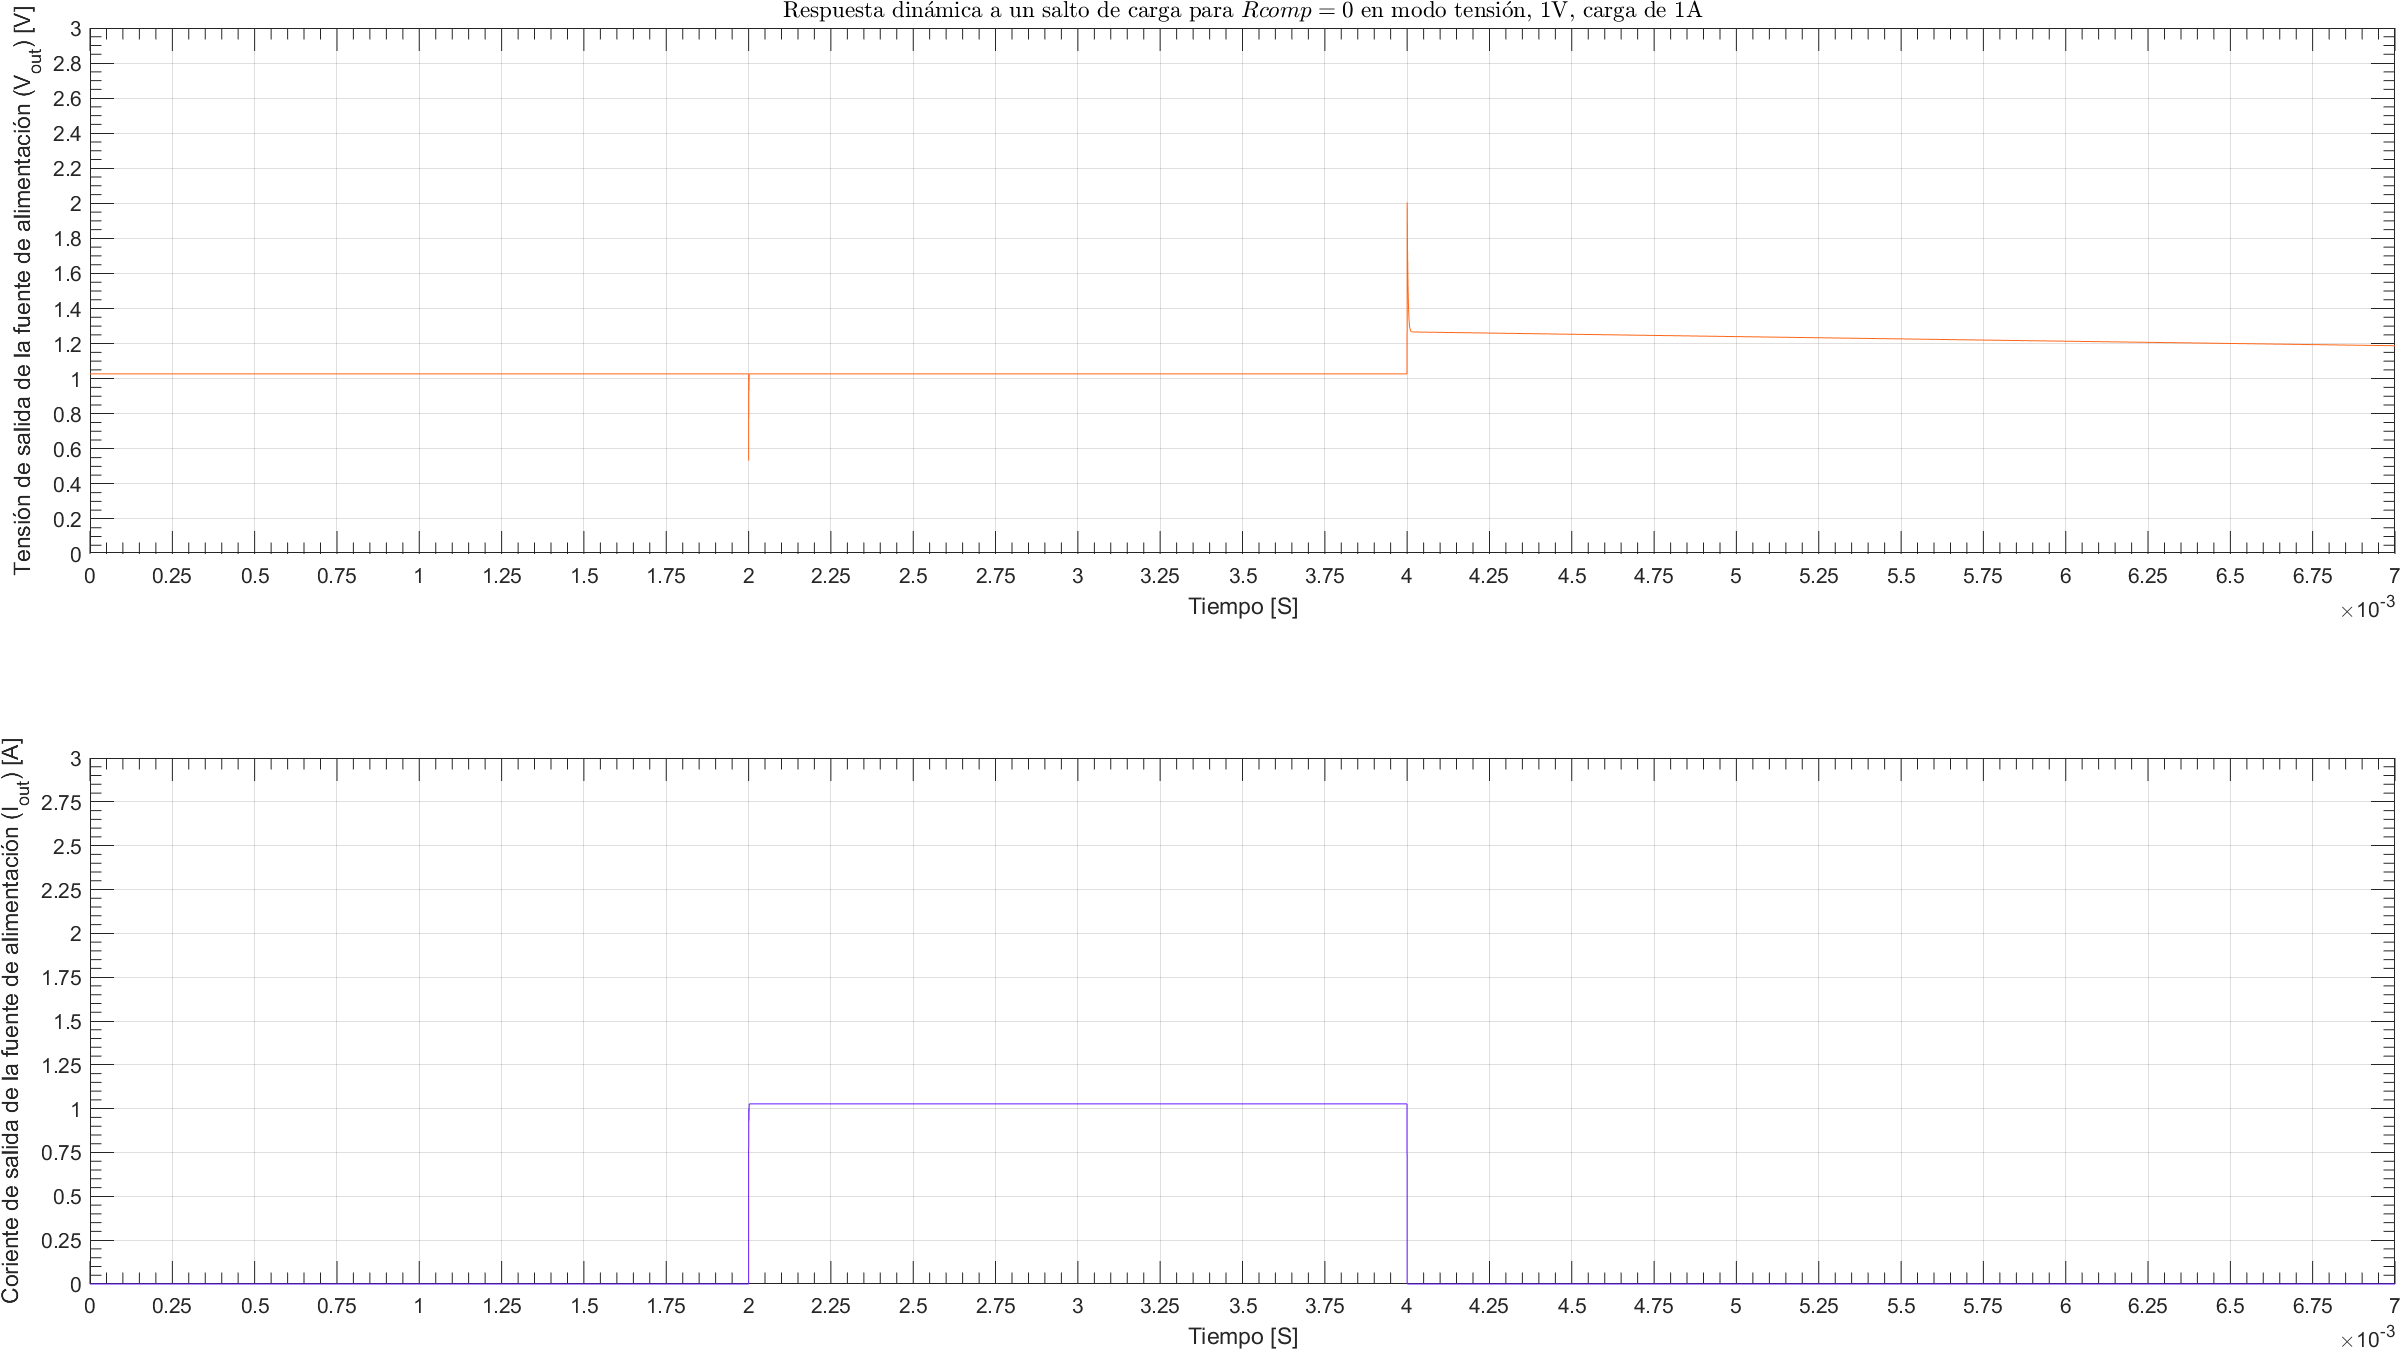
\includegraphics[width=1.1 \textwidth, angle=90]{./img/plots/dynamic/power_supply_RCOMP_0_STEP_Modo2.png}
\caption{\label{fig:fig_power_supply_RCOMP_STEP_0_Modo2}\footnotesize{Respuesta dinámica en modo tensión, $V_{out} = 1 \si[per-mode=symbol]{\volt}$, para $R_{comp} = 0 \si[per-mode=symbol]{\ohm} $.}}
\end{center}
\end{figure}

\clearpage

\begin{figure}[H] %htb
\begin{center}
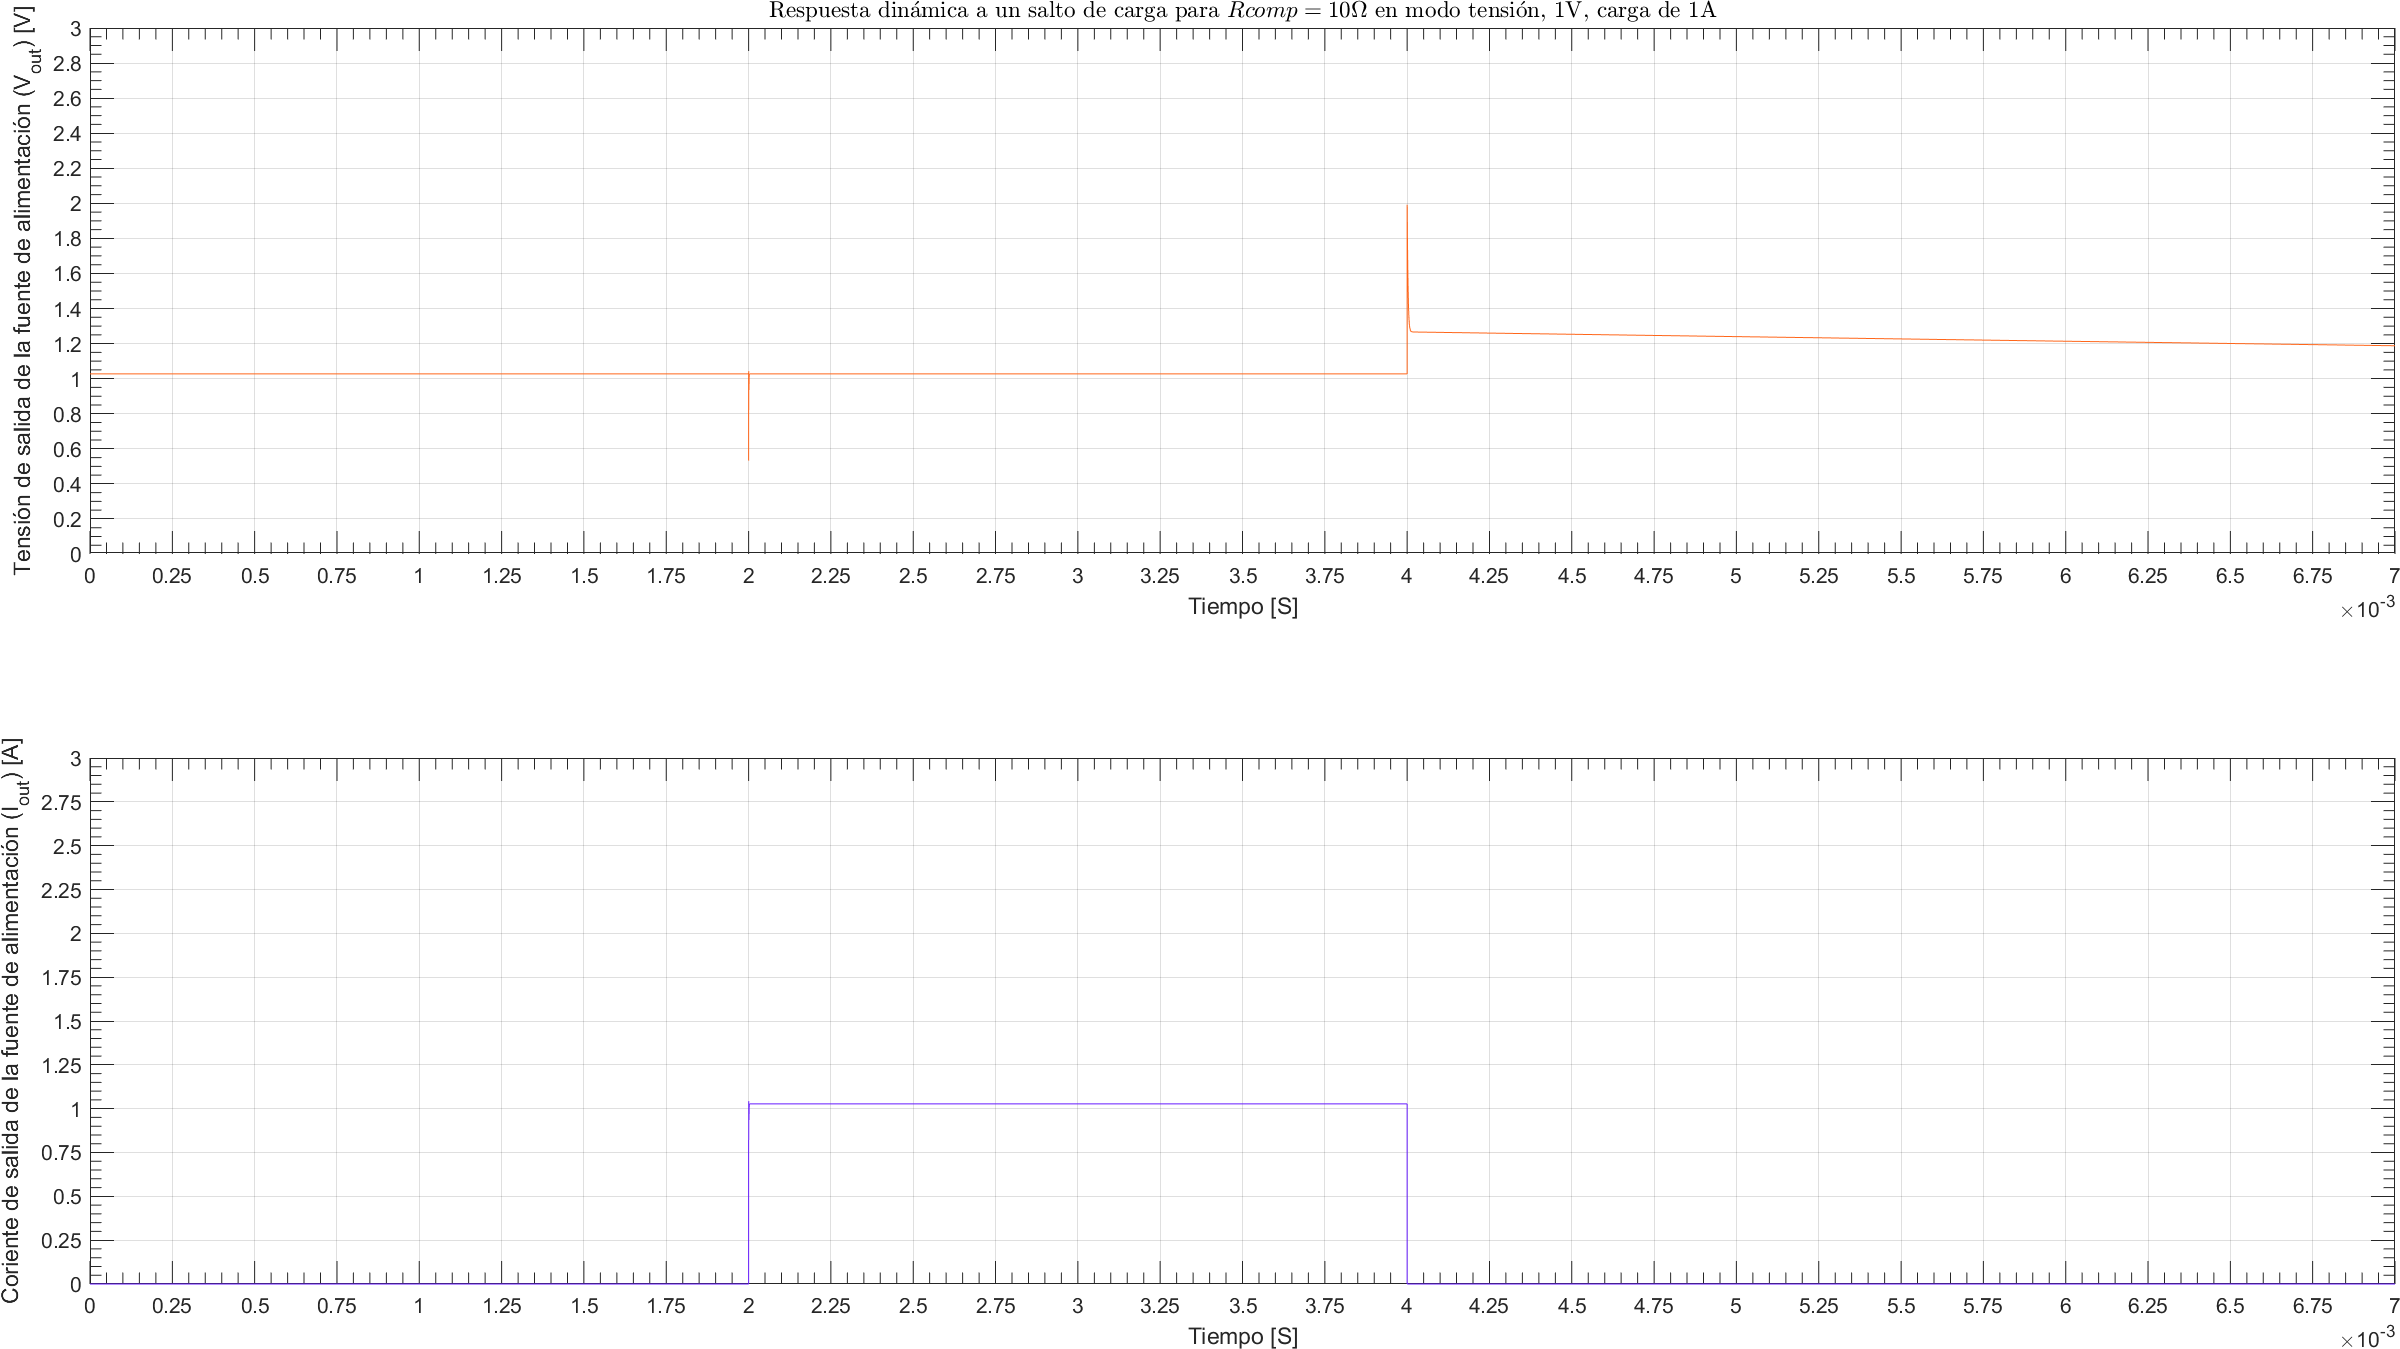
\includegraphics[width=1.1 \textwidth, angle=90]{./img/plots/dynamic/power_supply_RCOMP_10_STEP_Modo2.png}
\caption{\label{fig:fig_power_supply_RCOMP_STEP_10_Modo2}\footnotesize{Respuesta dinámica en modo tensión, $V_{out} = 1 \si[per-mode=symbol]{\volt}$, para $R_{comp} = 10 \si[per-mode=symbol]{\ohm} $.}}
\end{center}
\end{figure}

\clearpage

\begin{figure}[H] %htb
\begin{center}
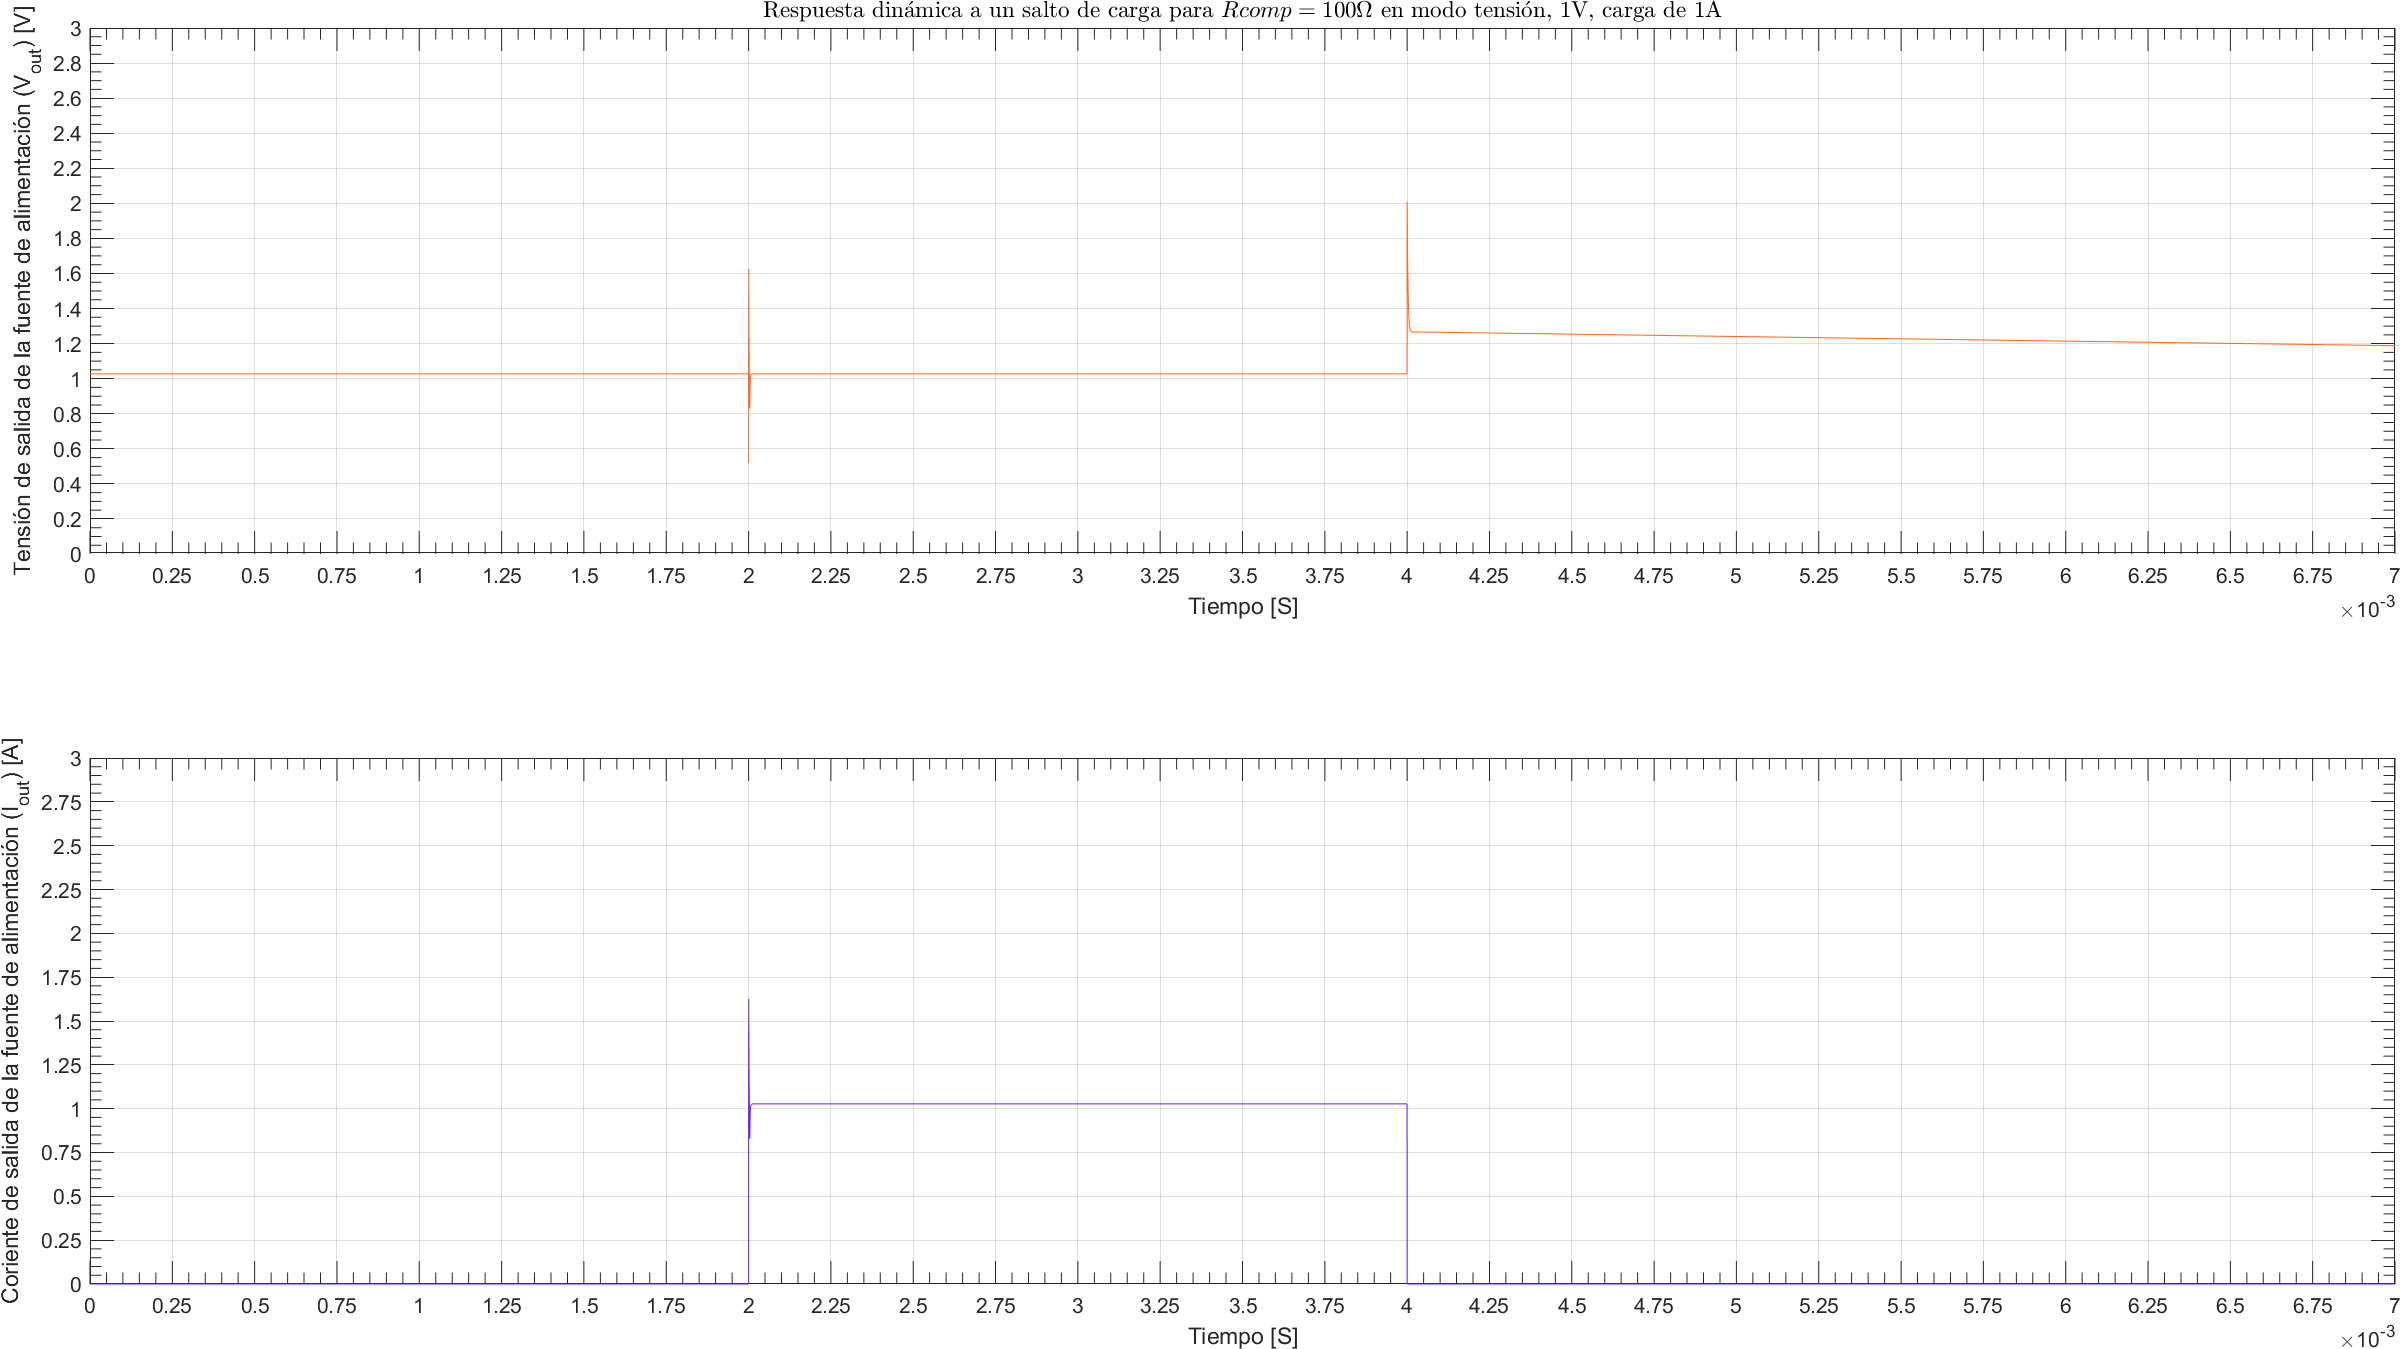
\includegraphics[width=1.1 \textwidth, angle=90]{./img/plots/dynamic/power_supply_RCOMP_100_STEP_Modo2.png}
\caption{\label{fig:fig_power_supply_RCOMP_STEP_100_Modo2}\footnotesize{Respuesta dinámica en modo tensión, $V_{out} = 1 \si[per-mode=symbol]{\volt}$, para $R_{comp} = 100 \si[per-mode=symbol]{\ohm} $.}}
\end{center}
\end{figure}

\clearpage


\subsubsection{Análisis para $R_{comp}$ en modo corriente, $I_{out} = 2 \si[per-mode=symbol]{\ampere}$, $R_{L} = 0 \si[per-mode=symbol]{\ohm}$}

Se puede ver en la figura~\figref{fig:fig_power_supply_RCOMP_LOOP_Modo3} como ya con el valor de $R_{comp} = 10 \si[per-mode=symbol]{\ohm}$ se logra unos margen de fase y ganancia muy buenos, valores de $R_{comp}$ por debajo o por arriba o empeoran los márgenes o presentan picos de resonancia en la respuesta en frecuencia, además que un valor mayor disminuye el ancho de banda, como se puede ver en la figura~\figref{fig:fig_power_supply_RCOMP_RF_Modo3}. A nivel de respuesta dinámica, no se ven grandes diferencias entre los valores simulados, ver figura~\figref{fig:fig_power_supply_RCOMP_STEP_0_Modo3}, figura~\figref{fig:fig_power_supply_RCOMP_STEP_10_Modo3} y figura~\figref{fig:fig_power_supply_RCOMP_STEP_100_Modo3}.

\vfill


% RCOMP MODO 3.

\clearpage

\begin{figure}[H] %htb
\begin{center}
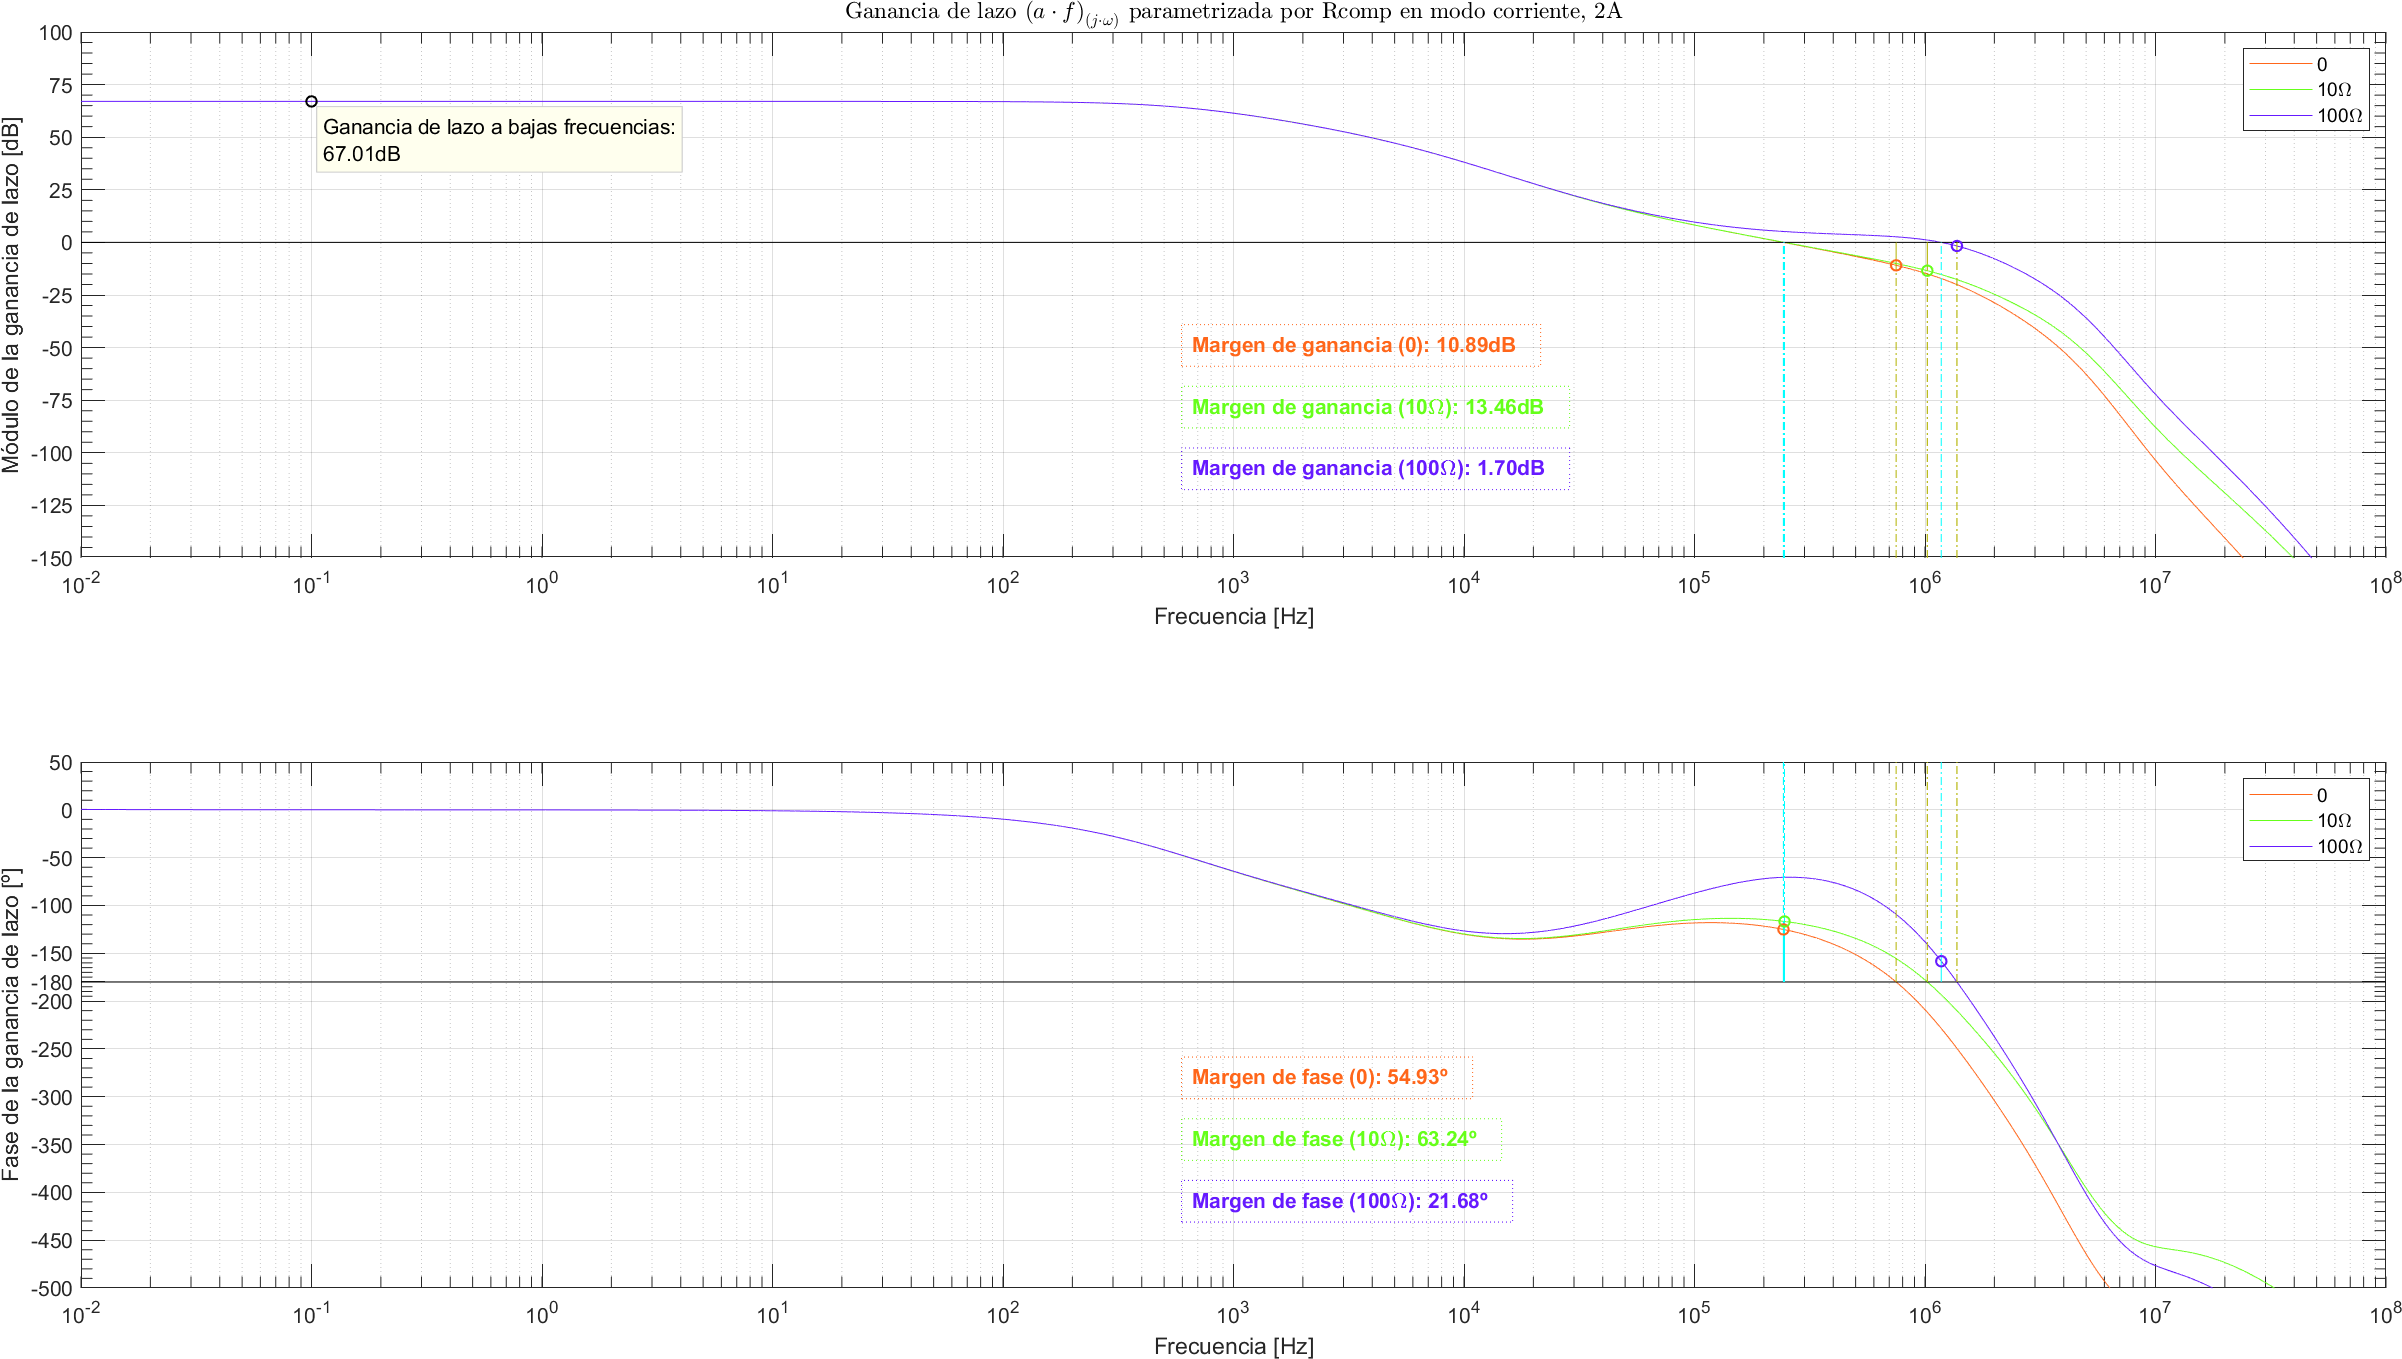
\includegraphics[width=1.1 \textwidth, angle=90]{./img/plots/loop/power_supply_RCOMP_LOOP_Modo3.png}
\caption{\label{fig:fig_power_supply_RCOMP_LOOP_Modo3}\footnotesize{Ganancia de lazo en modo corriente, $I_{out} = 2 \si[per-mode=symbol]{\ampere}$, en función de la frecuencia parametrizada por $R_{comp}$.}}
\end{center}
\end{figure}


\clearpage

\begin{figure}[H] %htb
\begin{center}
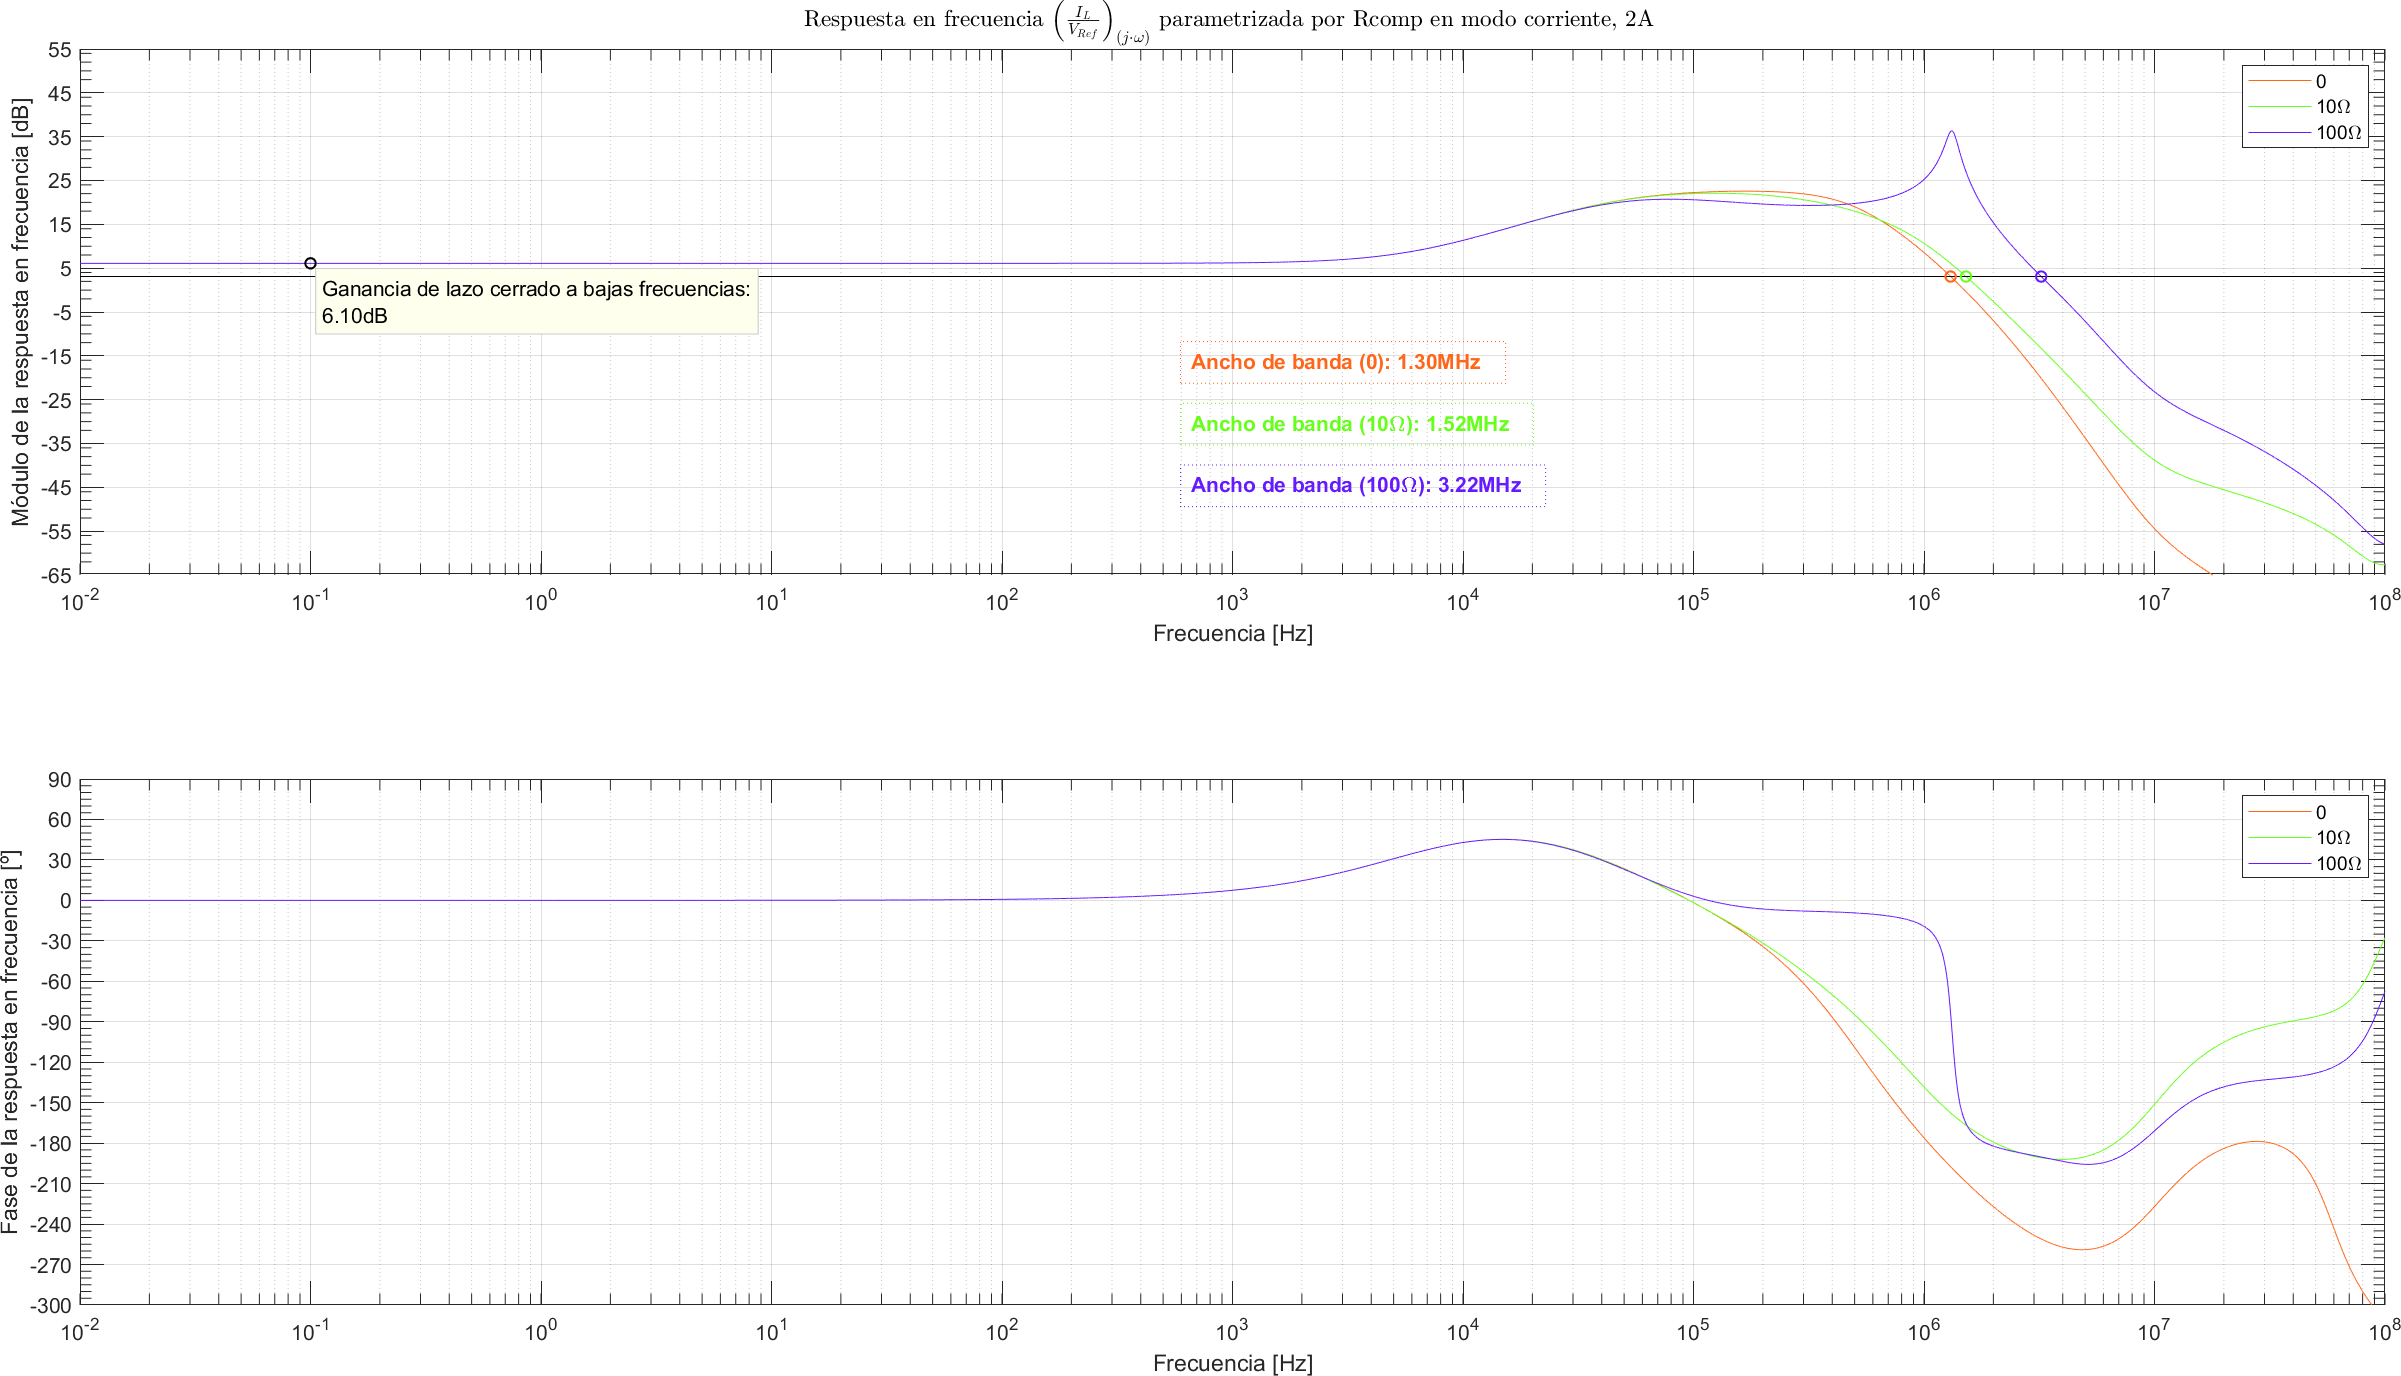
\includegraphics[width=1.1 \textwidth, angle=90]{./img/plots/rf/power_supply_RCOMP_RF_Modo3.png}
\caption{\label{fig:fig_power_supply_RCOMP_RF_Modo3}\footnotesize{Respuesta en frecuencia en modo corriente, $I_{out} = 2 \si[per-mode=symbol]{\ampere}$, en función de la frecuencia parametrizada por $R_{comp}$.}}
\end{center}
\end{figure}

\clearpage

\begin{figure}[H] %htb
\begin{center}
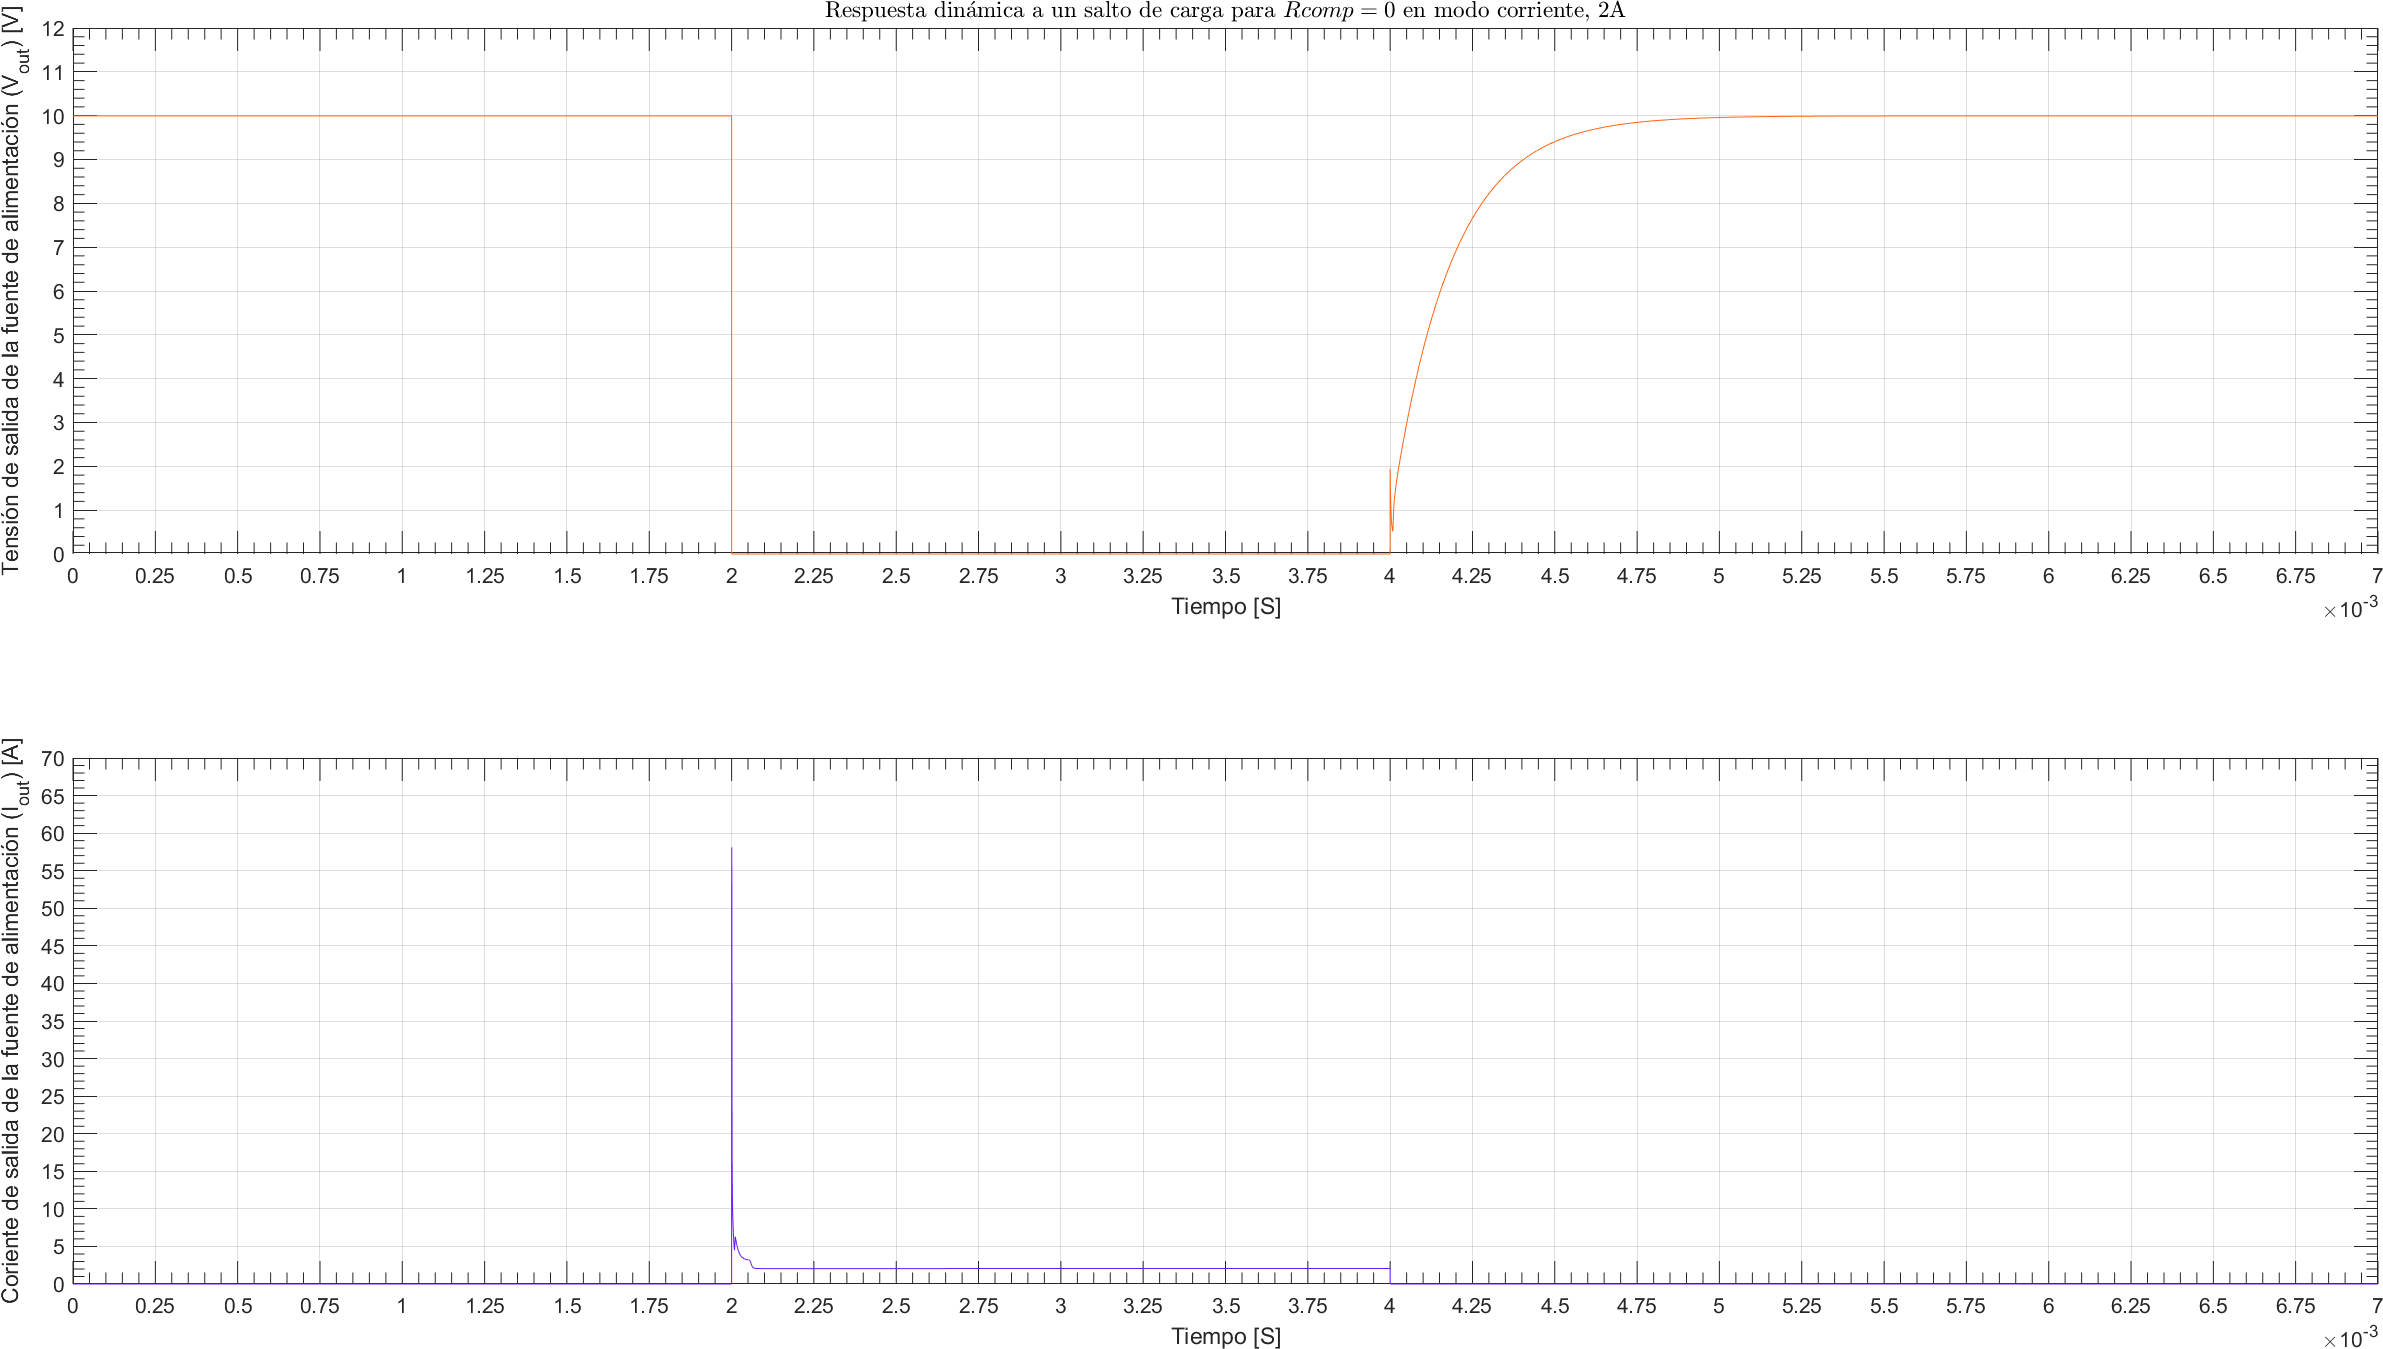
\includegraphics[width=1.1 \textwidth, angle=90]{./img/plots/dynamic/power_supply_RCOMP_0_STEP_Modo3.png}
\caption{\label{fig:fig_power_supply_RCOMP_STEP_0_Modo3}\footnotesize{Respuesta dinámica en modo corriente, $I_{out} = 2 \si[per-mode=symbol]{\ampere}$, para $R_{comp} = 0 \si[per-mode=symbol]{\ohm} $.}}
\end{center}
\end{figure}

\clearpage

\begin{figure}[H] %htb
\begin{center}
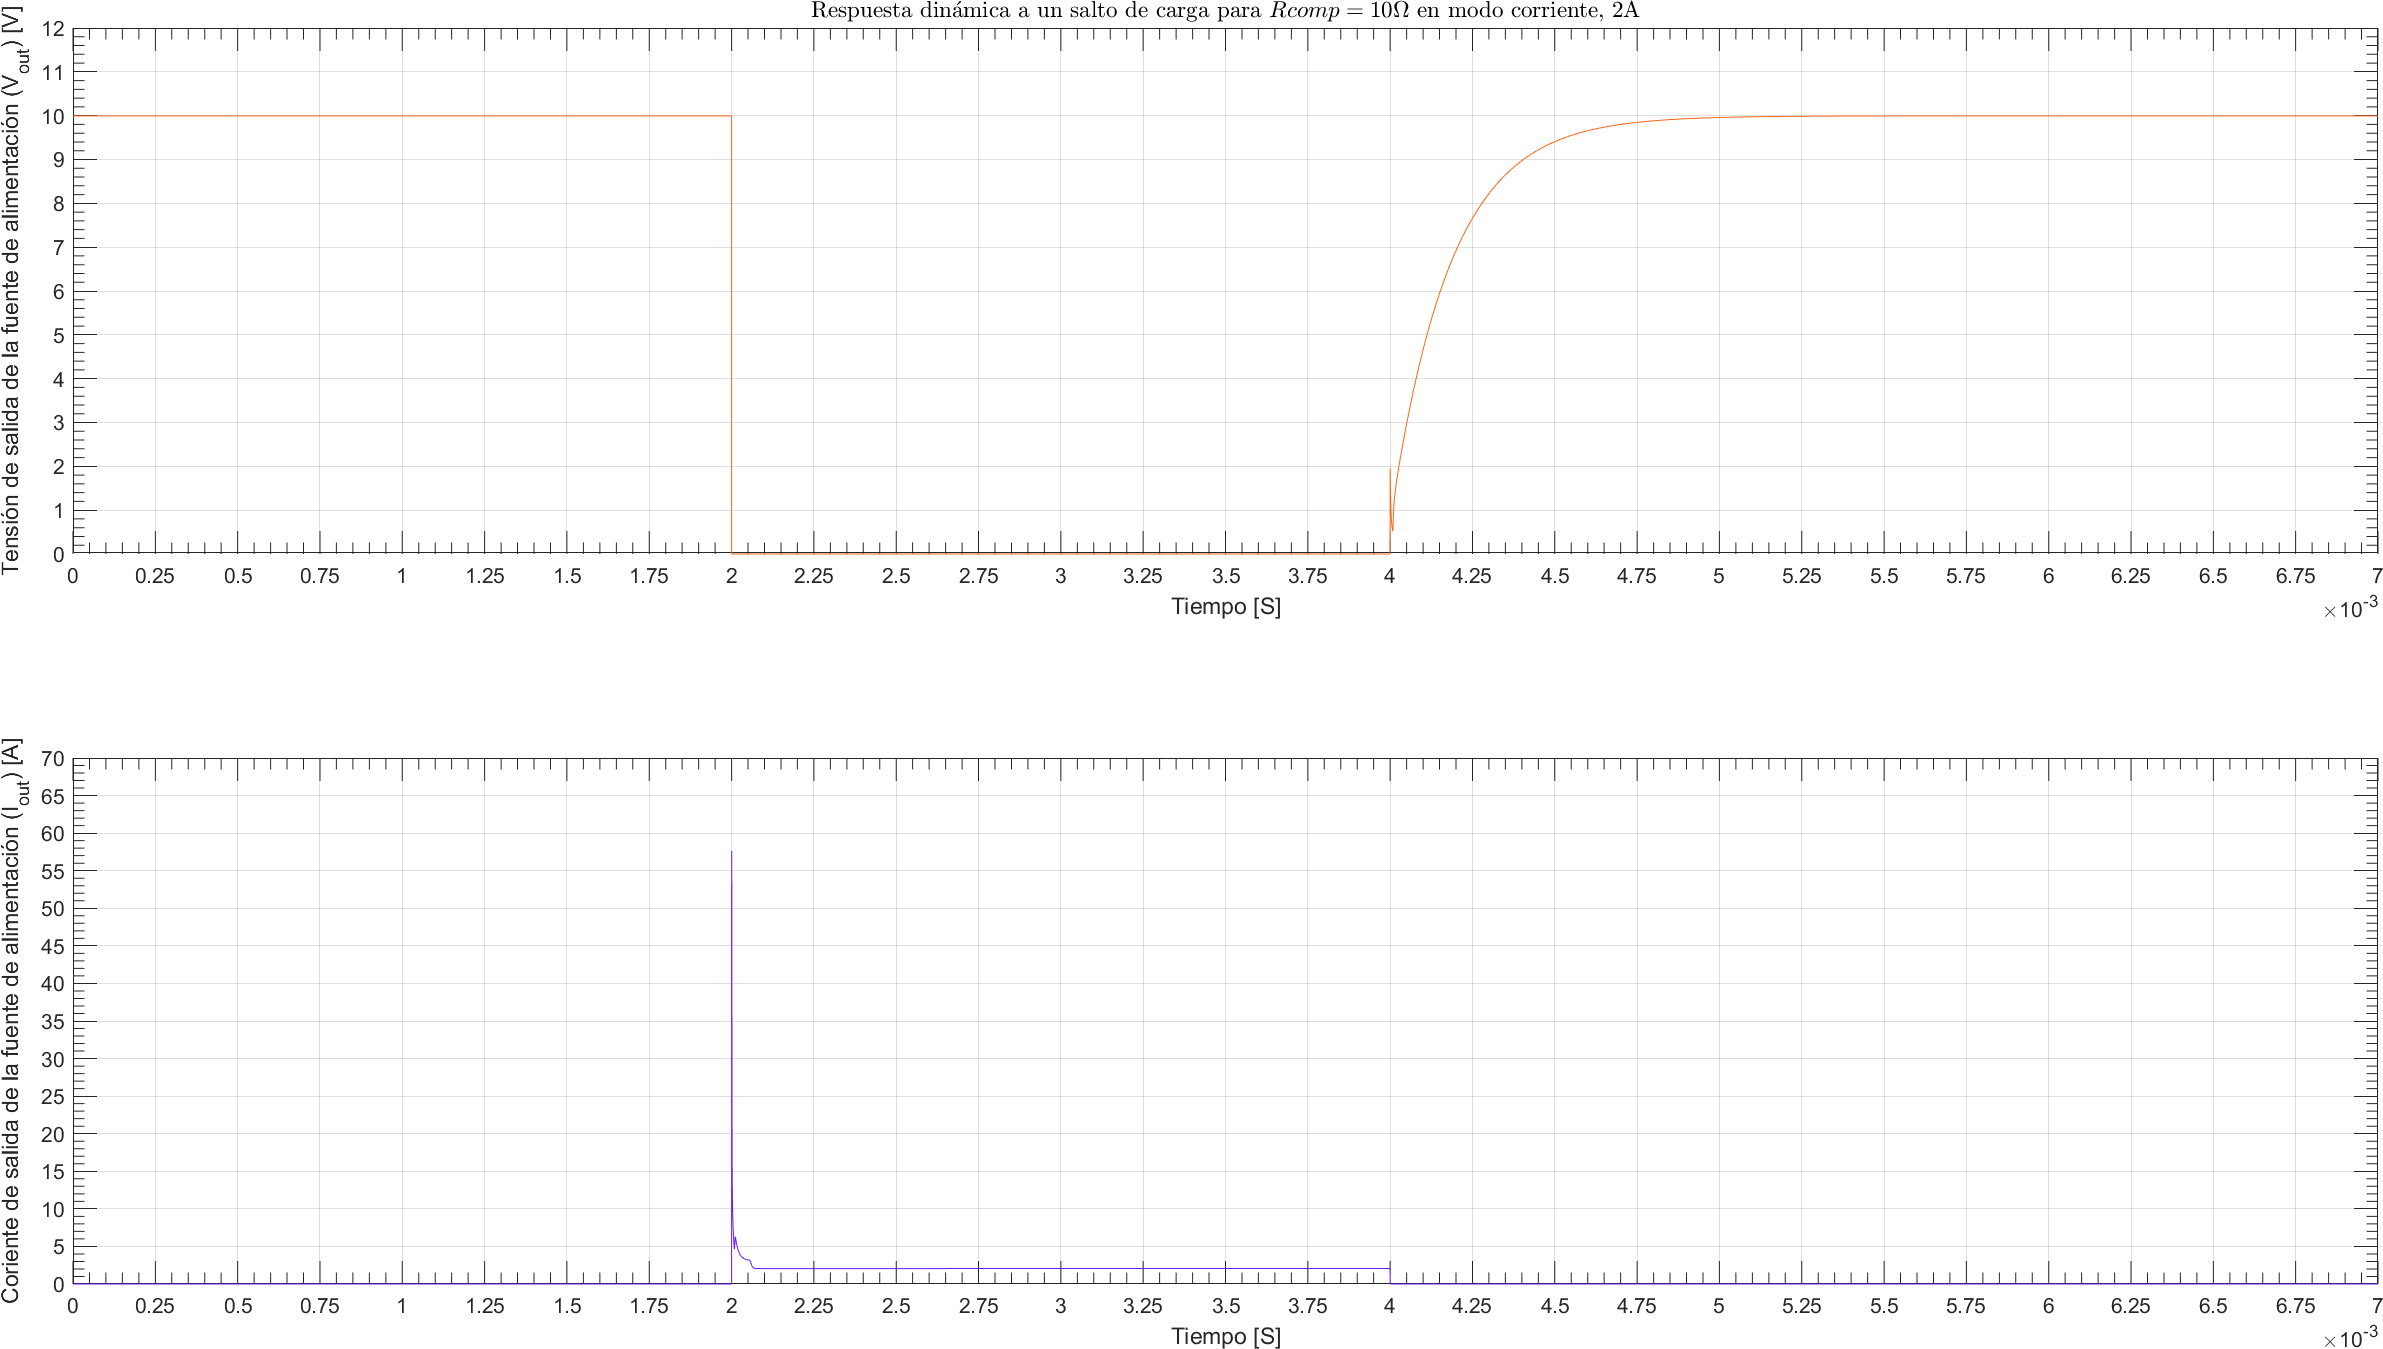
\includegraphics[width=1.1 \textwidth, angle=90]{./img/plots/dynamic/power_supply_RCOMP_10_STEP_Modo3.png}
\caption{\label{fig:fig_power_supply_RCOMP_STEP_10_Modo3}\footnotesize{Respuesta dinámica en modo corriente, $I_{out} = 2 \si[per-mode=symbol]{\ampere}$, para $R_{comp} = 10 \si[per-mode=symbol]{\ohm} $.}}
\end{center}
\end{figure}

\clearpage

\begin{figure}[H] %htb
\begin{center}
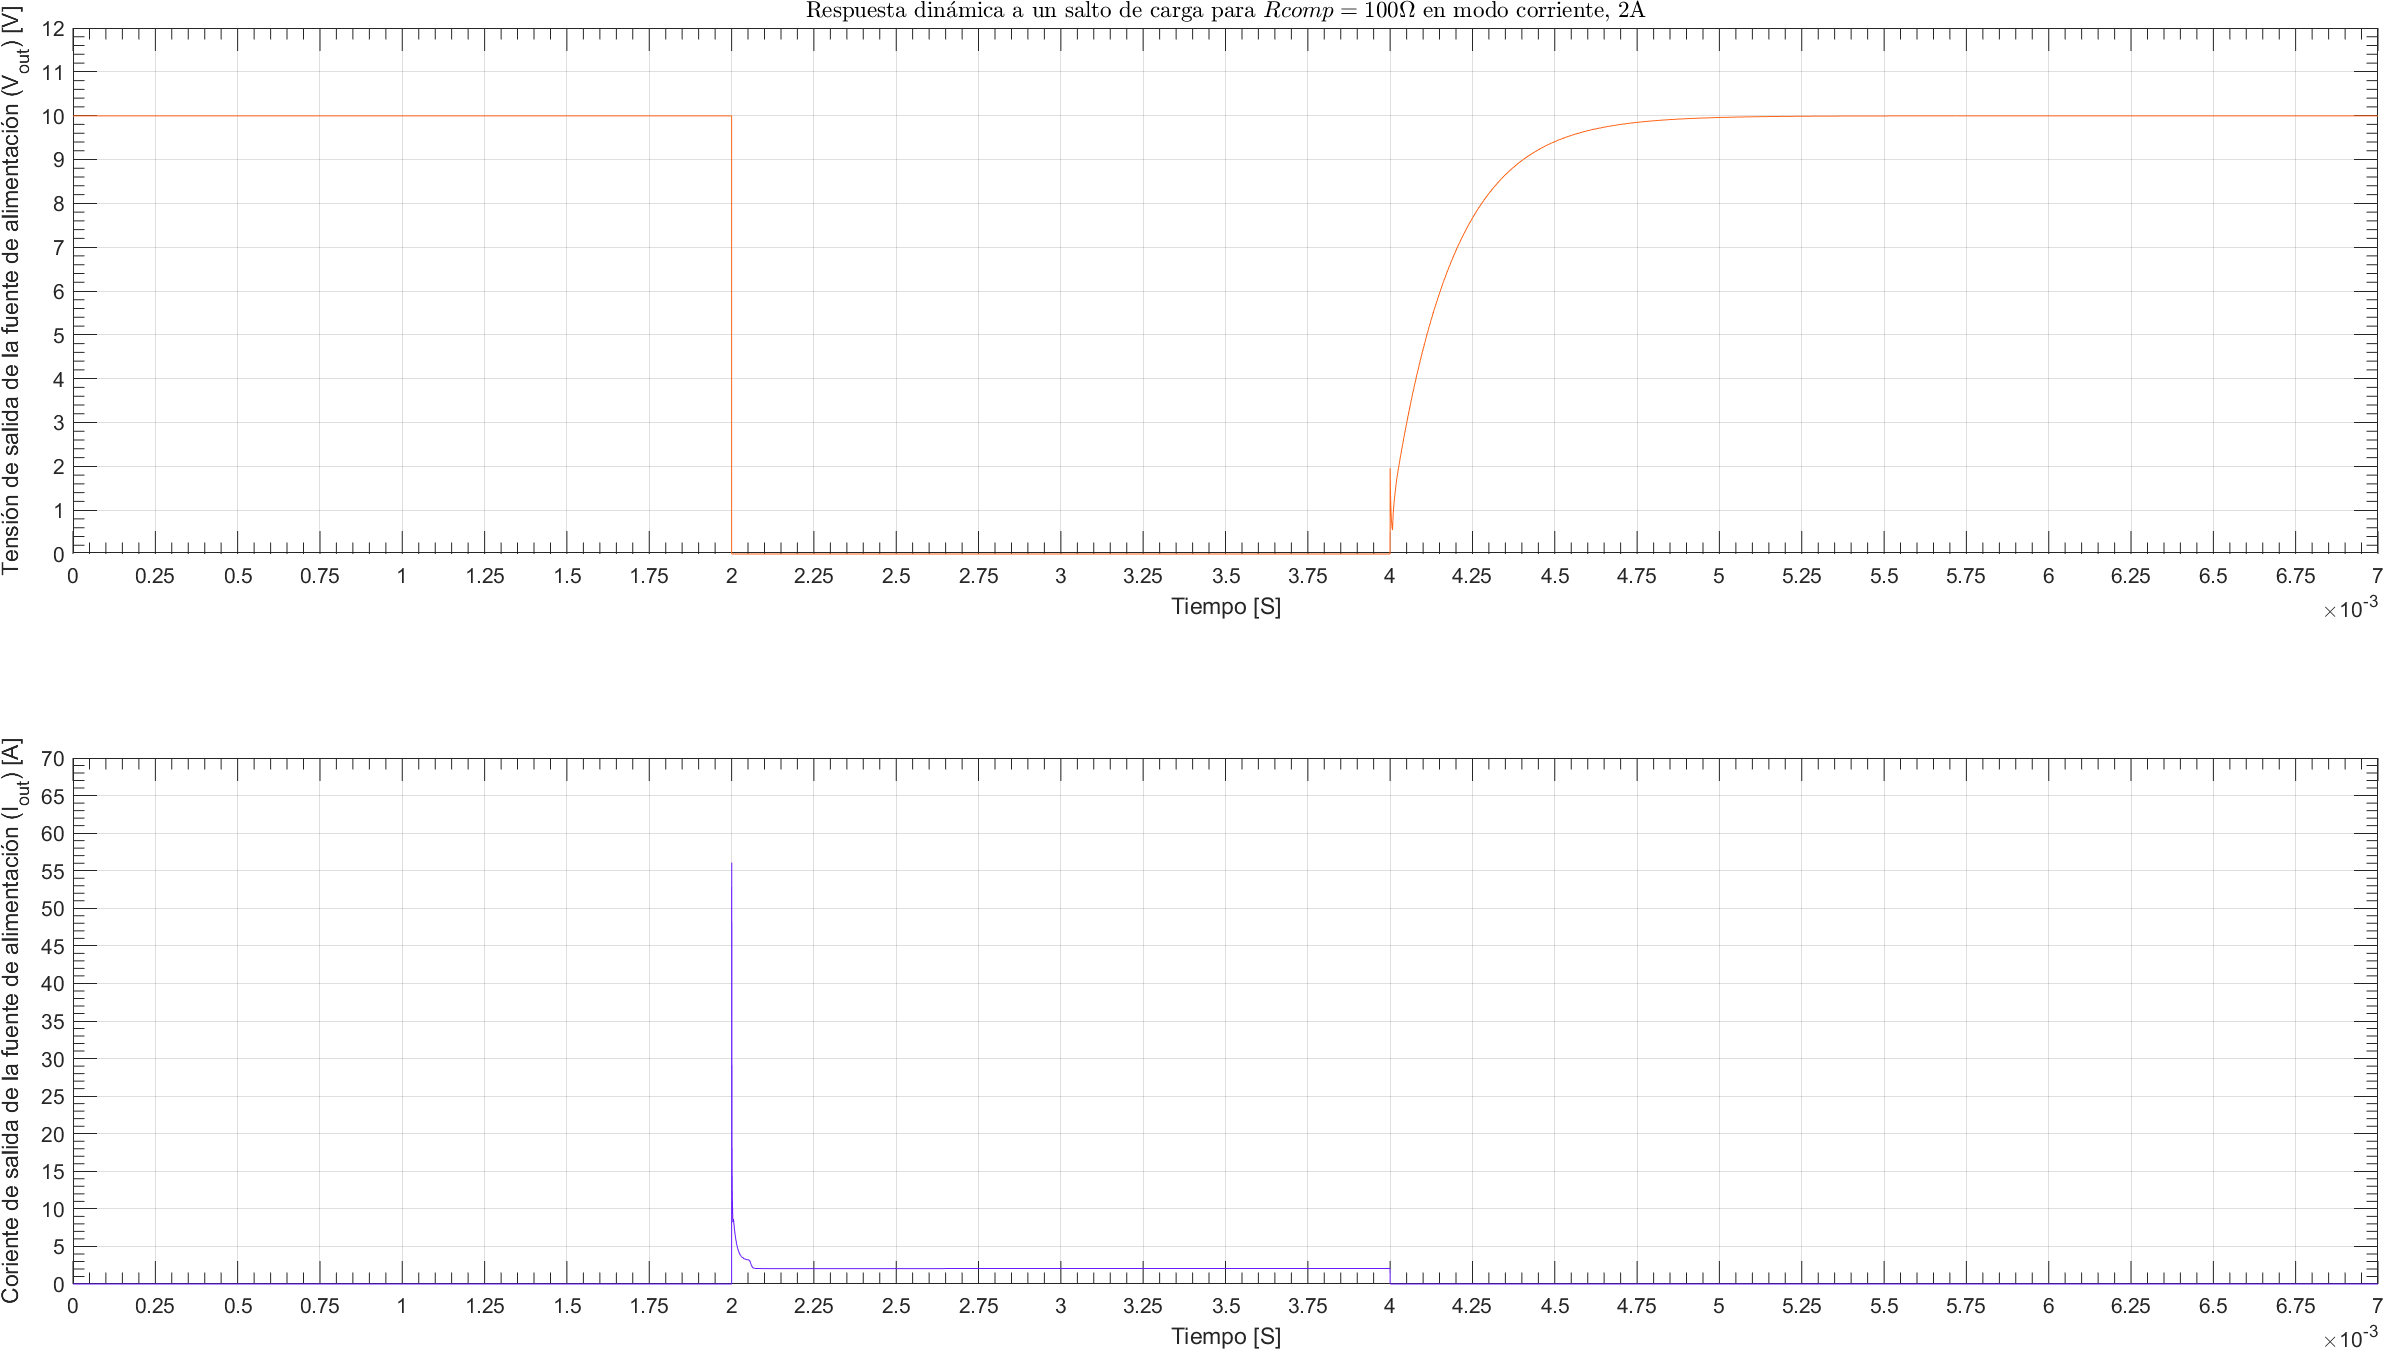
\includegraphics[width=1.1 \textwidth, angle=90]{./img/plots/dynamic/power_supply_RCOMP_100_STEP_Modo3.png}
\caption{\label{fig:fig_power_supply_RCOMP_STEP_100_Modo3}\footnotesize{Respuesta dinámica en modo corriente, $I_{out} = 2 \si[per-mode=symbol]{\ampere}$, para $R_{comp} = 100 \si[per-mode=symbol]{\ohm} $.}}
\end{center}
\end{figure}

\clearpage


\subsubsection{Análisis para $R_{comp}$ en modo corriente, $I_{out} = 200 \si[per-mode=symbol]{\milli\ampere}$, $R_{L} = 0 \si[per-mode=symbol]{\ohm}$}
Se puede ver en la figura~\figref{fig:fig_power_supply_RCOMP_LOOP_Modo4} como ya con el valor de $R_{comp} = 10 \si[per-mode=symbol]{\ohm}$ se logra unos margen de fase y ganancia muy buenos, valores de $R_{comp}$ por debajo o por arriba o empeoran los márgenes o presentan picos de resonancia en la respuesta en frecuencia, además que un valor mayor disminuye el ancho de banda, como se puede ver en la figura~\figref{fig:fig_power_supply_RCOMP_RF_Modo4}. A nivel de respuesta dinámica, no se ven grandes diferencias entre los valores simulados, ver figura~\figref{fig:fig_power_supply_RCOMP_STEP_0_Modo4}, figura~\figref{fig:fig_power_supply_RCOMP_STEP_10_Modo4} y figura~\figref{fig:fig_power_supply_RCOMP_STEP_100_Modo4}.

\vfill


%  RCOMP MODO 4.

\clearpage

\begin{figure}[H] %htb
\begin{center}
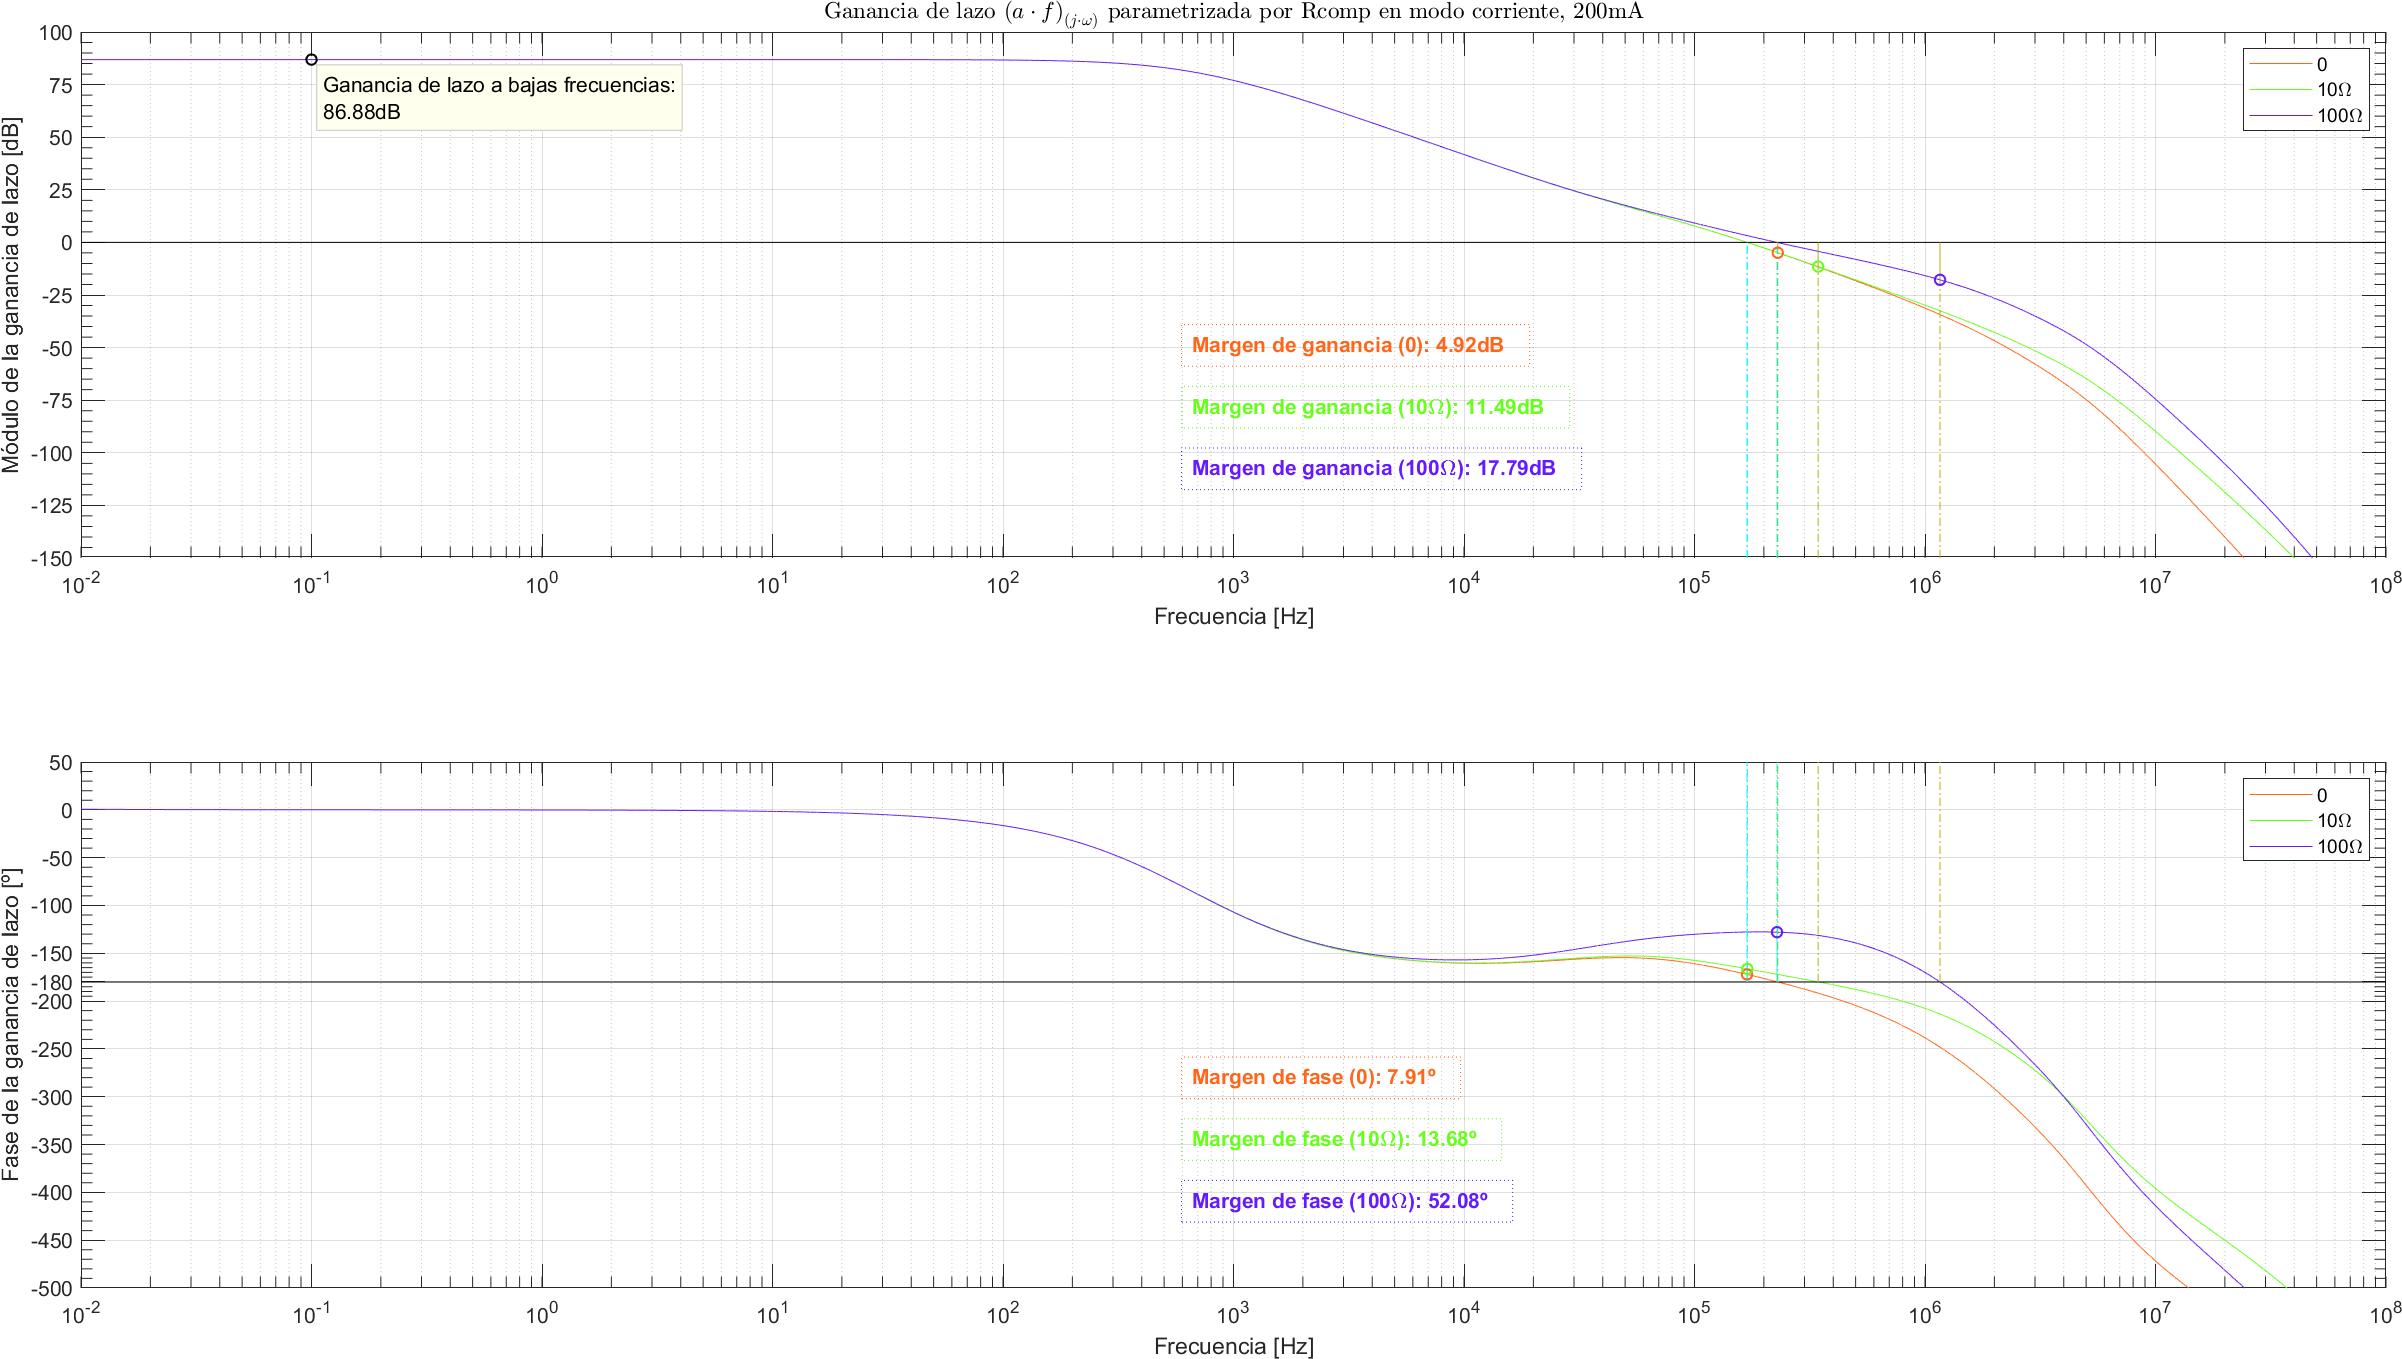
\includegraphics[width=1.1 \textwidth, angle=90]{./img/plots/loop/power_supply_RCOMP_LOOP_Modo4.png}
\caption{\label{fig:fig_power_supply_RCOMP_LOOP_Modo4}\footnotesize{Ganancia de lazo en modo corriente, $I_{out} = 200 \si[per-mode=symbol]{\milli\ampere}$, en función de la frecuencia parametrizada por $R_{comp}$.}}
\end{center}
\end{figure}


\clearpage

\begin{figure}[H] %htb
\begin{center}
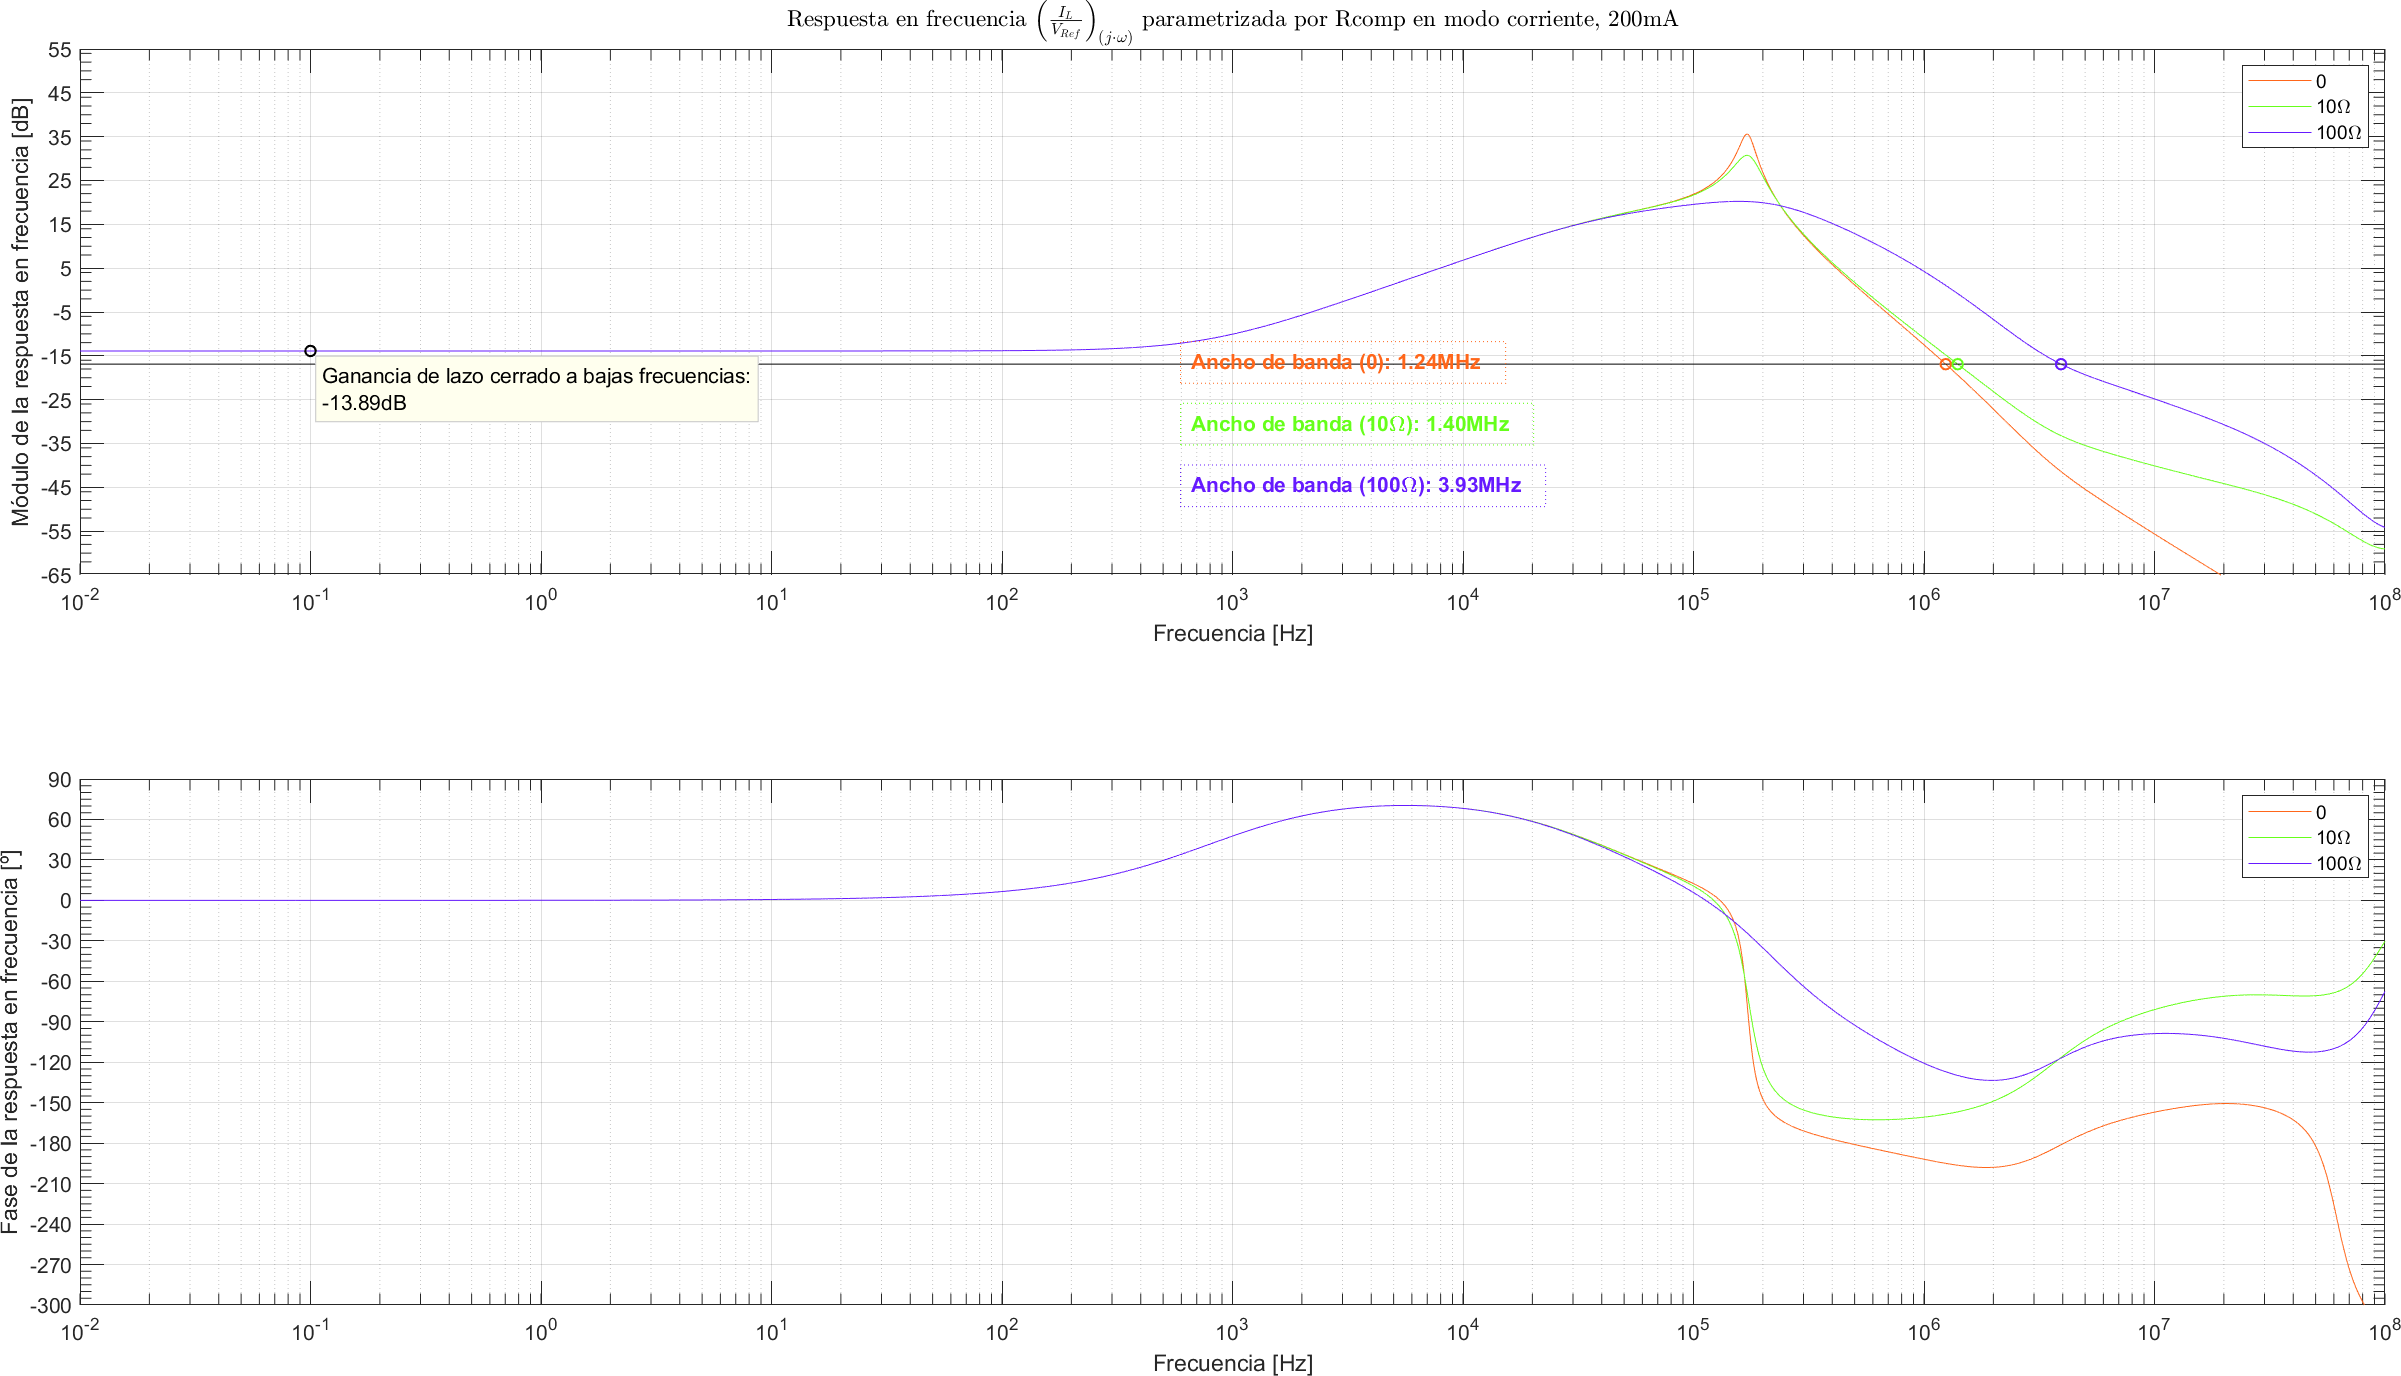
\includegraphics[width=1.1 \textwidth, angle=90]{./img/plots/rf/power_supply_RCOMP_RF_Modo4.png}
\caption{\label{fig:fig_power_supply_RCOMP_RF_Modo4}\footnotesize{Respuesta en frecuencia en modo corriente, $I_{out} = 200 \si[per-mode=symbol]{\milli\ampere}$, en función de la frecuencia parametrizada por $R_{comp}$.}}
\end{center}
\end{figure}

\clearpage

\begin{figure}[H] %htb
\begin{center}
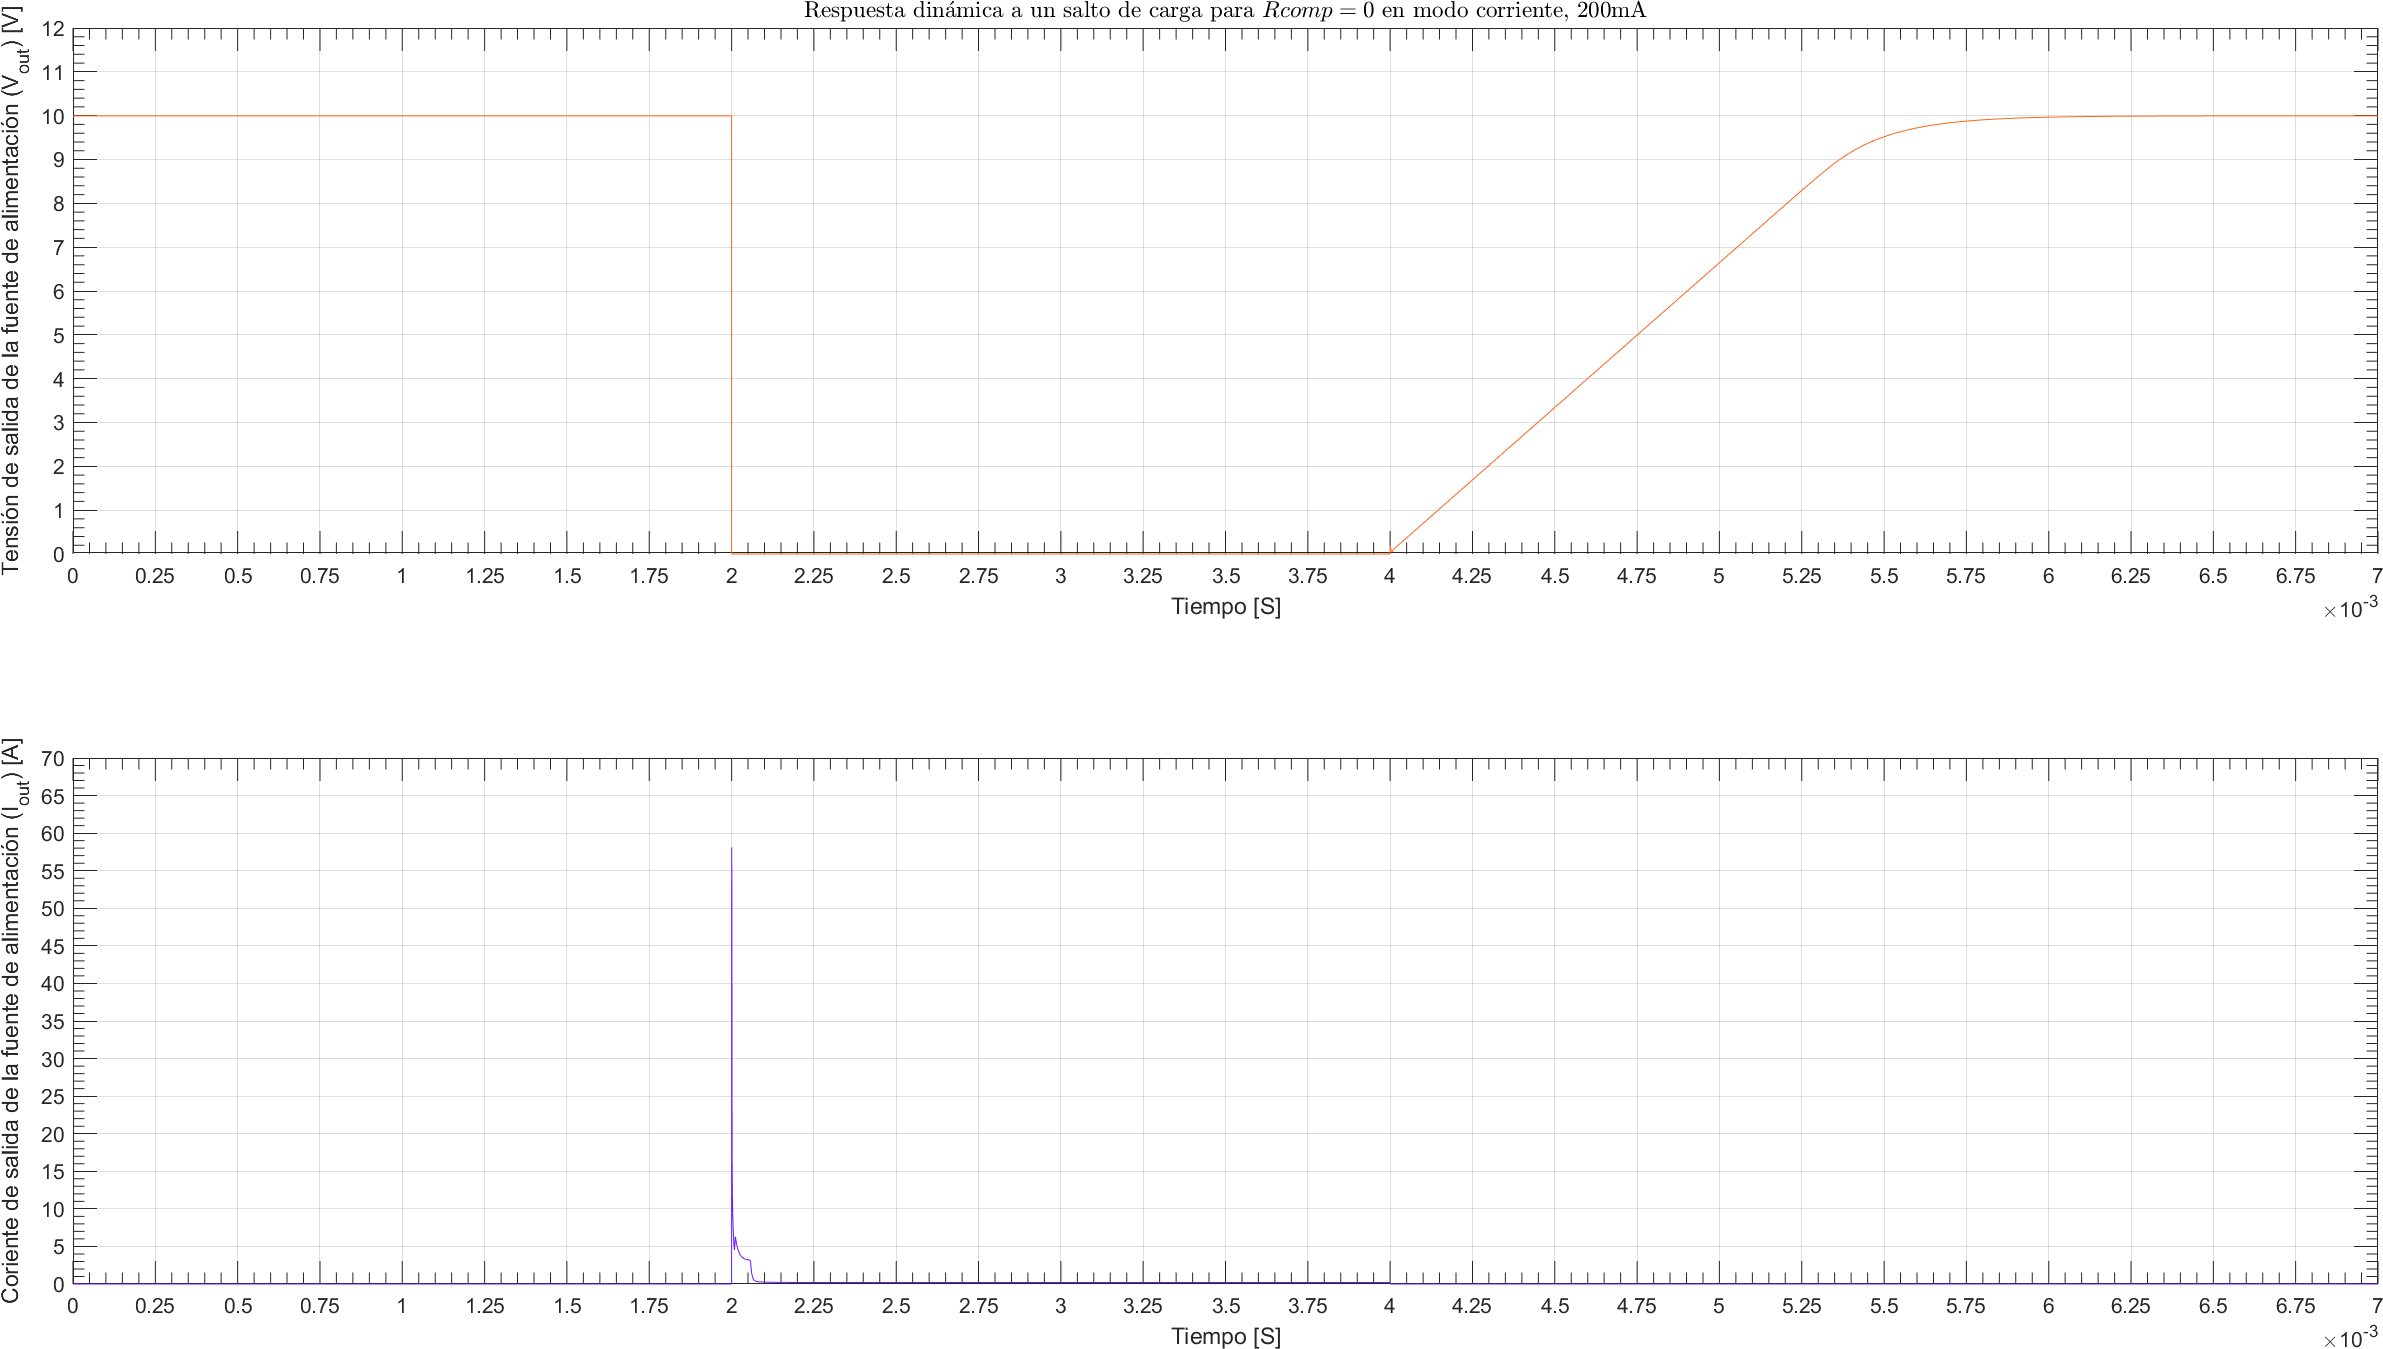
\includegraphics[width=1.1 \textwidth, angle=90]{./img/plots/dynamic/power_supply_RCOMP_0_STEP_Modo4.png}
\caption{\label{fig:fig_power_supply_RCOMP_STEP_0_Modo4}\footnotesize{Respuesta dinámica en modo corriente, $I_{out} = 200 \si[per-mode=symbol]{\milli\ampere}$, para $R_{comp} = 0 \si[per-mode=symbol]{\ohm} $.}}
\end{center}
\end{figure}

\clearpage

\begin{figure}[H] %htb
\begin{center}
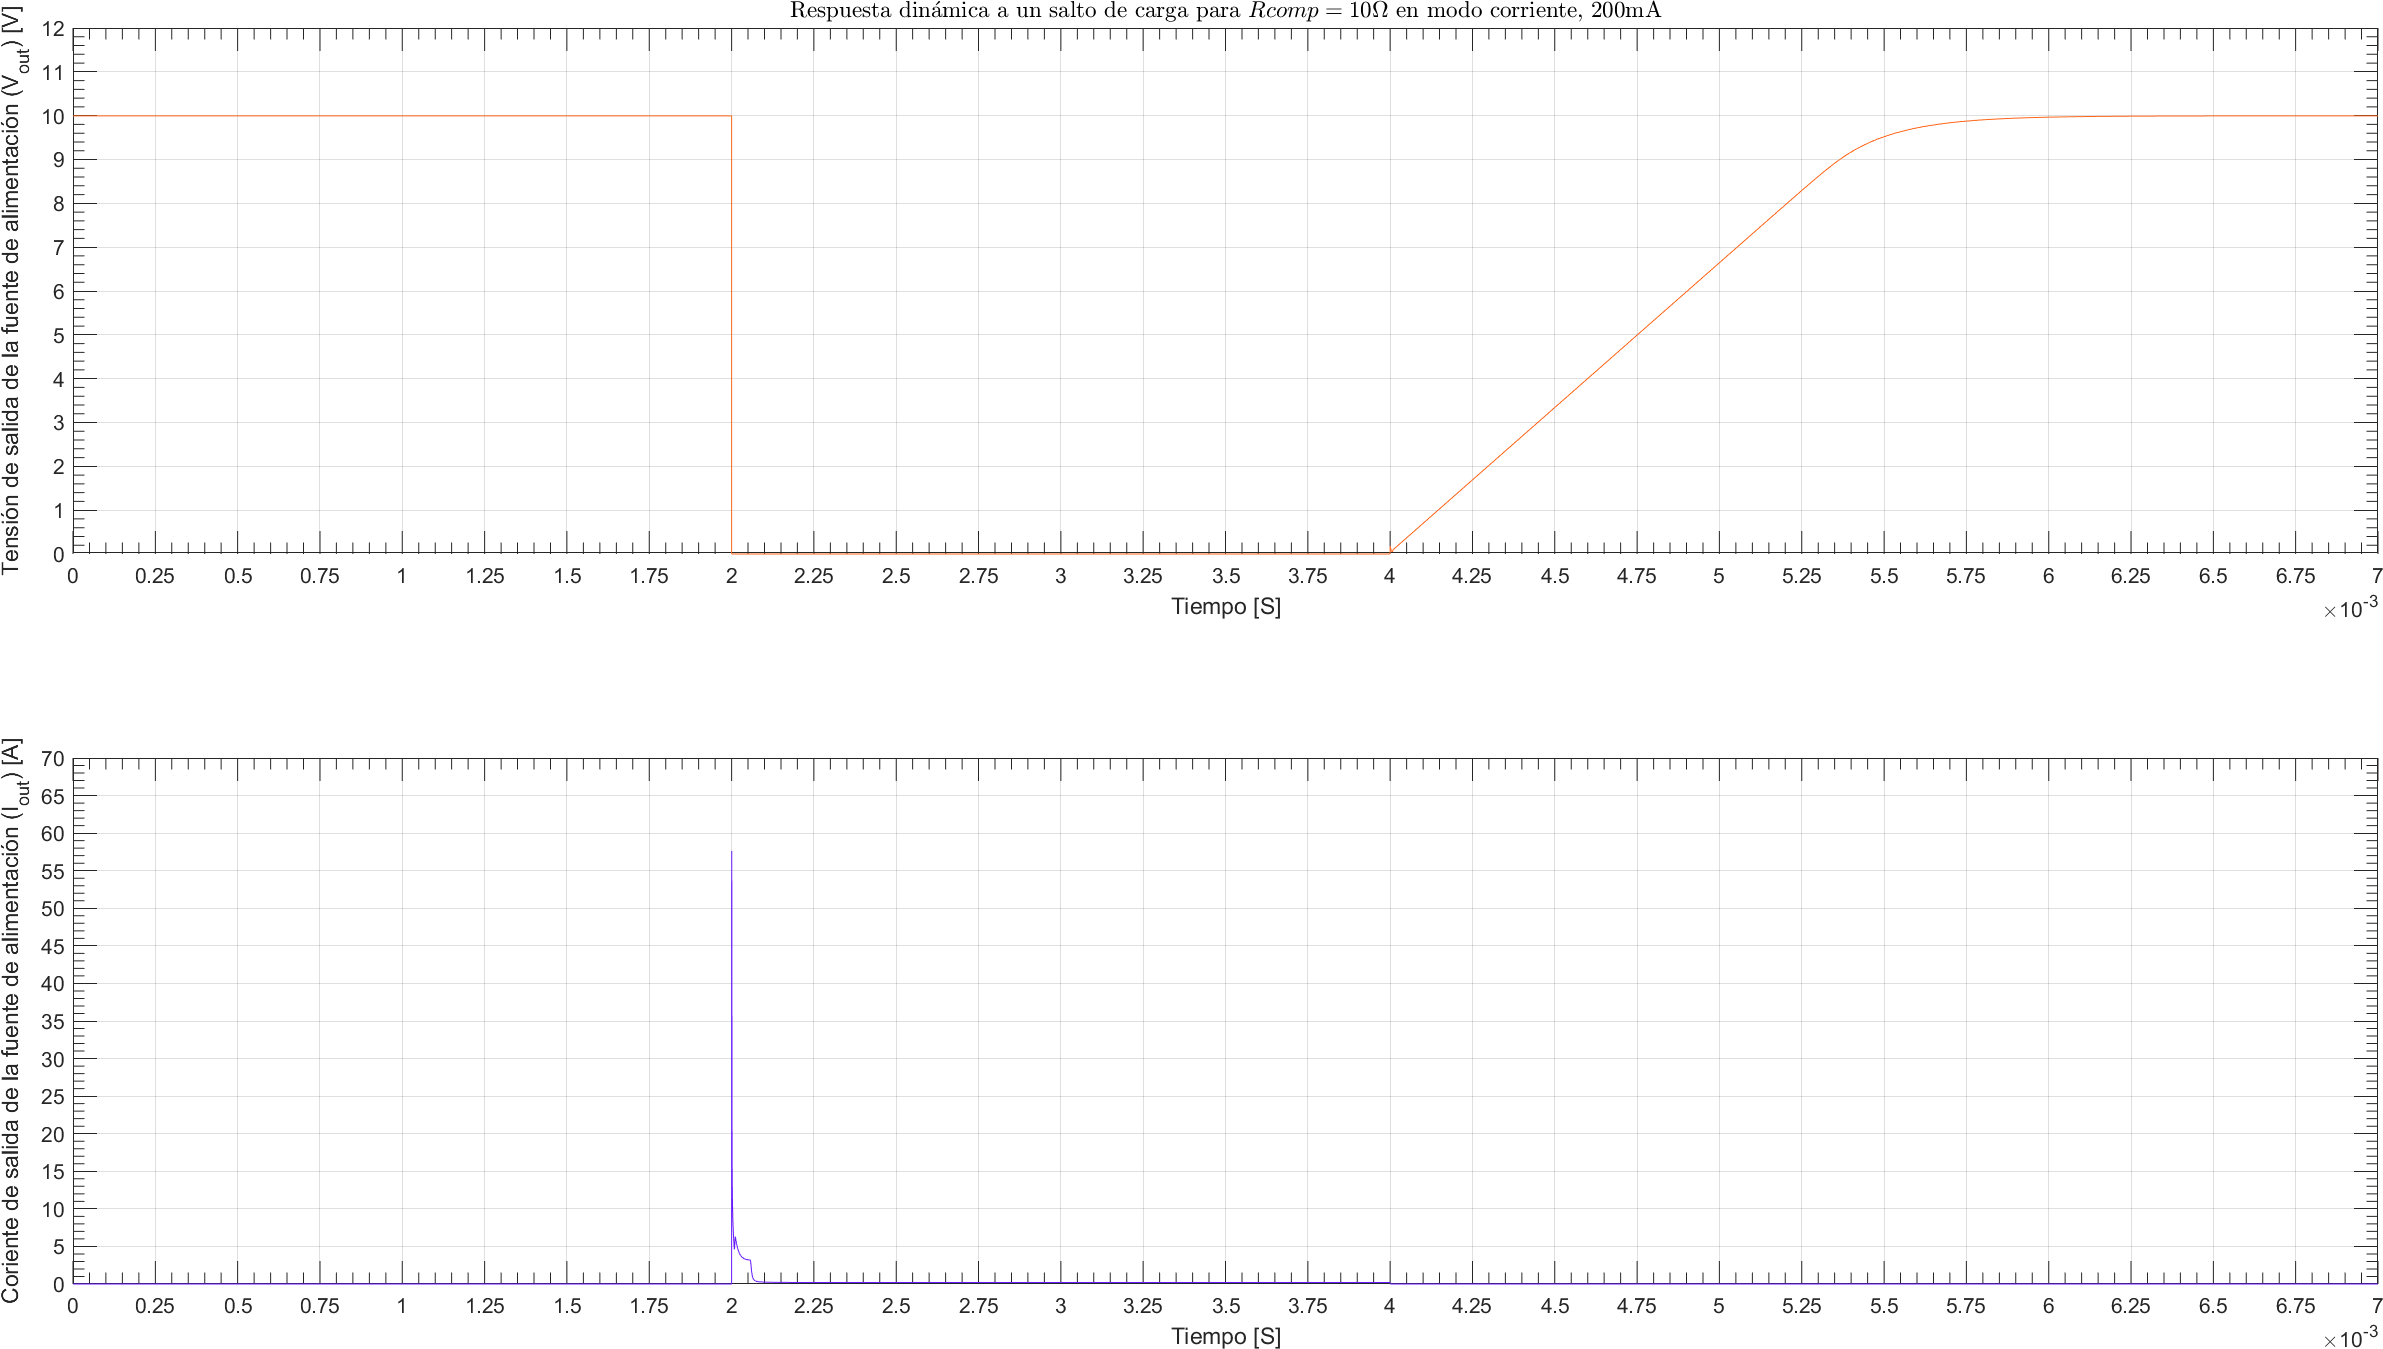
\includegraphics[width=1.1 \textwidth, angle=90]{./img/plots/dynamic/power_supply_RCOMP_10_STEP_Modo4.png}
\caption{\label{fig:fig_power_supply_RCOMP_STEP_10_Modo4}\footnotesize{Respuesta dinámica en modo corriente, $I_{out} = 200 \si[per-mode=symbol]{\milli\ampere}$, para $R_{comp} = 10 \si[per-mode=symbol]{\ohm} $.}}
\end{center}
\end{figure}

\clearpage

\begin{figure}[H] %htb
\begin{center}
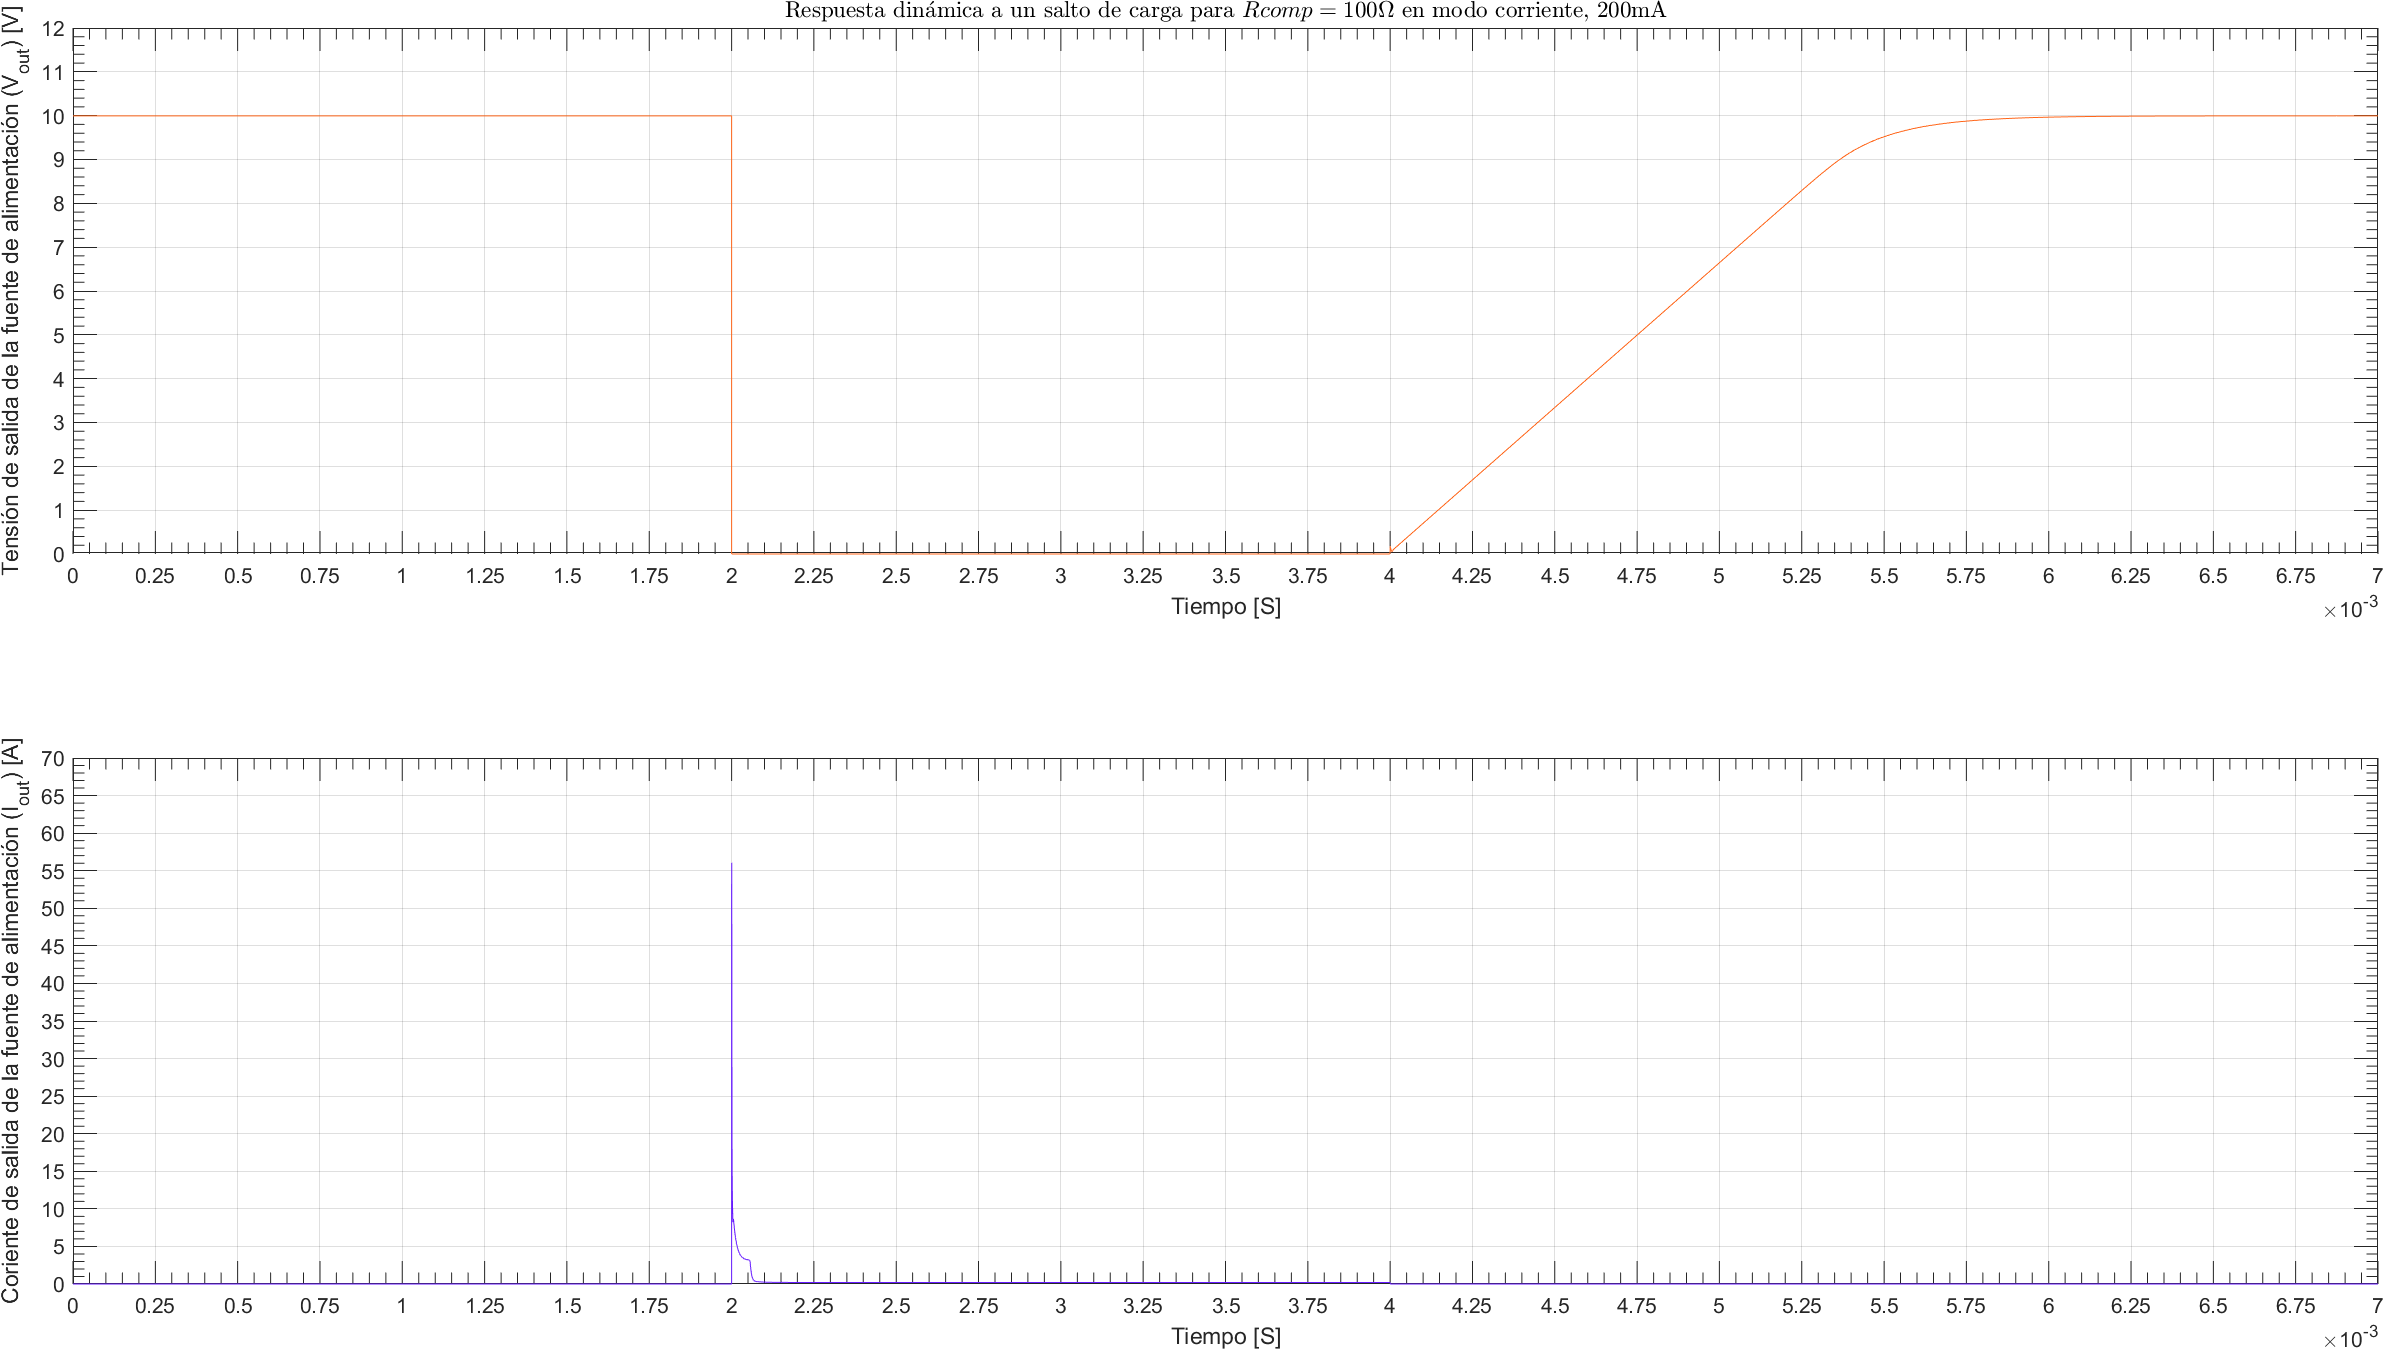
\includegraphics[width=1.1 \textwidth, angle=90]{./img/plots/dynamic/power_supply_RCOMP_100_STEP_Modo4.png}
\caption{\label{fig:fig_power_supply_RCOMP_STEP_100_Modo4}\footnotesize{Respuesta dinámica en modo corriente, $I_{out} = 200 \si[per-mode=symbol]{\milli\ampere}$, para $R_{comp} = 100 \si[per-mode=symbol]{\ohm} $.}}
\end{center}
\end{figure}

\clearpage




